
 %\textcolor[rgb]{0.00,0.07,1.00}{\uline{}}

\documentclass[%
 aip,jap,
% jmp,
% bmf,
% sd,
% rsi,
 amsmath,amssymb,
%preprint,%
 reprint,%
% floatfix,
%author-year,%
%author-numerical,%
% Conference Proceedings
]{revtex4-1}

\usepackage{graphicx}% Include figure files
\usepackage{dcolumn}% Align table columns on decimal point
\usepackage{bm}% bold math
%\usepackage[mathlines]{lineno}% Enable numbering of text and display math
%\linenumbers\relax % Commence numbering lines

\usepackage[utf8]{inputenc}
\usepackage[T1]{fontenc}
\usepackage{mathptmx}
\usepackage{etoolbox}
\usepackage{color}
\usepackage[normalem]{ulem} % для подчёркиваний uline
\usepackage{multirow}

%% Apr 2021: AIP requests that the corresponding
%% email to be moved after the affiliations
\makeatletter
\def\@email#1#2{%
 \endgroup
 \patchcmd{\titleblock@produce}
  {\frontmatter@RRAPformat}
  {\frontmatter@RRAPformat{\produce@RRAP{*#1\href{mailto:#2}{#2}}}\frontmatter@RRAPformat}
  {}{}
}%
\makeatother
\begin{document}

%\preprint{AIP/123-QED}

\title[FeB transformations under ultrasound loading]{Features of FeB pair light-induced dissociation and repair in silicon $n^+$-$p$-$p^+$ structures under ultrasound loading}
%Sample Title:\\with Forced Linebreak}
% Force line breaks with \\
\author{O. Olikh}
 \email{olegolikh@knu.ua}
 \affiliation{Physics Faculty, Taras Shevchenko National University of Kyiv, Kyiv, Ukraine.}%Lines break automatically or can be forced with \\
\author{V. Kostylyov}%
% \email{Second.Author@institution.edu.}
\author{V. Vlasiuk}
\author{R. Korkishko}
\author{Ya. Olikh}
\affiliation{
V. Lashkaryov Institute of Semiconductor Physics of NAS of Ukraine, Kyiv, Ukraine%\\This line break forced with \textbackslash\textbackslash
}%

\author{R. Chupryna}
\affiliation{Physics Faculty, Taras Shevchenko National University of Kyiv, Kyiv, Ukraine.}

%\author{C. Author}
% \homepage{http://www.Second.institution.edu/~Charlie.Author.}
%\affiliation{%
%Second institution and/or address%\\This line break forced% with \\
%}%

\date{\today}% It is always \today, today,
             %  but any date may be explicitly specified

%\begin{abstract}
%The influence of ultrasound on iron--boron pair dissociation and association in silicon $n^+$–$p$-$p^+$ structures were investigated experimentally.
%The FeB pair transformations were monitored by measurements of  short circuit current kinetics.
%It was found that ultrasound causes the decrease in both the concentration of pairs, which were dissociated by light, and time of association.
%The phenomenon was investigated at different light intensities, temperatures, frequencies, and power of ultrasound loading.
%The possible mechanisms underlying the revealed  effects were analyzed.
%\end{abstract}

\begin{abstract}
\textcolor[rgb]{0.00,0.07,1.00}{\uline{
The experimental research in ultrasound impact on iron--boron pair transformation in
silicon $n^+$–$p$-$p^+$ structures has revealed the decrease in concentration of pairs dissociated by light, as well as in the time of pair associations.}}
The FeB pair  \textcolor[rgb]{0.00,0.07,1.00}{\uline{changes}} were monitored by measuring short circuit current kinetics.
The \textcolor[rgb]{0.00,0.07,1.00}{\uline{ultrasound influence}} was investigated at different light intensities, temperatures,
frequencies and power of \textcolor[rgb]{0.00,0.07,1.00}{\uline{acoustic wave}}.
The possible mechanisms underlying the revealed  effects were analyzed.
\end{abstract}

\maketitle


\section{\label{sec:Int}Introduction}

It is of wide knowledge that the properties of semiconducting crystals and structures are determined very much by their impurity compositions.
As a result, the methods aimed at modifying the system of defects are very important for practical applications.
Most \textcolor[rgb]{0.00,0.07,1.00}{\uline{of these}} methods use irradiation, thermal treatment, or specific conditions of crystal growth.
However, numerous experiments show that ultrasound also represents a sufficiently effective instrument to control the semiconductor defects.
For example, it has been found that the acoustic waves cause
spatial redistribution of defects,\cite{Roman:2010JAP,GORB2020,Ostapenko1999,Zaveryukhin2002,Zaver:2008,OstapSC}
transformation of metastable point defects,\cite{buyanova1994,Ostrovskii2001,Wosinski}
recharging of recombination centers,\cite{Olikh:Ultras,Korotchenkov1995}
and low temperature annealing of radiation defects.\cite{Podolian2012,YOlikh2006TPL,UST:OstrovCsI,Parchinskii2006,UST:LED_SM}
The effects of this kind are observed in particular in silicon, which is the basic modern material used in microelectronics and solar power engineering. \cite{Roman:2010JAP,GORB2020,Zaver:2008,Roman:2007APL,OlikhJAP,Ostrovskii2001,Podolian2012,Parchinskii2006}


\textcolor[rgb]{0.00,0.07,1.00}{\uline{
The advantages of using active ultrasound (US) are the}}
local action of elastic oscillations
and possibility to adjust the external impact by changing the type, polarization, or frequency of acoustic waves.\cite{Olikh2018JAP}
However, this method of modifying defect system has not found wide application not least because of the lack of appropriate experimental research.
In our opinion, it is most promising to use US loading (USL) as an additional factor of influence during various technological processes, which causes, in particular, the transformations in the defect system.
This assumption is supported by the results obtained during ion implantation performed in the US field.\cite{Roman:2010JAP,Roman:2007APL,Roman:2006JAP}


Iron is an important impurity in silicon--based integrated circuit and solar cell technology.
Most often, iron-related defects are the main recombination centers that determine the lifetime of  minority charge carriers in particular and device characteristics in general.
Therefore, the methods aimed at iron gettering at various stocks have practical importance.
\textcolor[rgb]{0.00,0.07,1.00}{\uline{
There are quite many reports concerning defects of this kind.}}
It is known that in thermal equilibrium at room temperature virtually all Fe$_i$ is present as Fe$_i$B$_s$ pairs in Si:B.\cite{FeBLight2,FeBJAP2005}
FeB pair dissociation can be accomplished by illumination at room temperature, by minority carrier injection, or by increasing the temperature.\cite{FeBLight2,FeBAssJAP2014,FeB_Zong}
Moreover, ultrasound  vibrations with the frequency of $25-80$~kHz and acoustic
\textcolor[rgb]{0.00,0.07,1.00}{\uline{
strain of $10^{-5}-10^{-4}$ (Cz--Si\cite{Ostapenko1995})
or $10^{-6}-10^{-5}$ (poly--Si \cite{Ostapenko1995SST,Ostapenko1994APL})
}}
are capable of destroying FeB pairs.
In practice, however, the most widely used technique is light-induced dissociation.
The peculiarities of the dissociation and subsequent repair are well studied.\cite{FeBLight2,FeBKin2019,FeBAssJAP2014,FeBJAP2005,FeBAssSST2011,lauer2016,FeBStrongIll,FeBkinAPL2008,FeBKinAPL2013}
However, to the best of our knowledge, there are no reports about US impact on these processes.

\textcolor[rgb]{0.00,0.07,1.00}{\uline{
Our aim was}} to study experimentally the influence of ultrasound loading ($2-30$~MHz)
on the processes of $\mathrm{FeB}\leftrightarrow\mathrm{Fe}_i+\mathrm{B}_s$ transformations in silicon solar cells (SCs).
 \textcolor[rgb]{0.00,0.07,1.00}{\uline{In order to prevent irreversible changes in the material properties, we used subthreshold intensity (strain $<2\cdot10^{-6}$)}}.
The obtained results can be \textcolor[rgb]{0.00,0.07,1.00}{\uline{applied}} for subtle acoustically controlled tuning of the processes involved in iron atom gettering.


\section{\label{sec:Exp}Experimental and calculation details}


The $n^+$-$p$-$p^+$-Si samples used in the experiment are shown in Fig.~\ref{Fig:sample}.
The structure was fabricated from a 380~$\mu$m thick $p$-type boron-doped
Czochralski silicon wafer with [100] orientation and resistivity of 10~Ohm$\cdot$cm.
The $n^+$ emitter with surface resistance of about $20-30$~$\Omega/\Box$
and  thickness of $0.7$~$\mu$m was formed by phosphorus diffusion \textcolor[rgb]{0.00,0.07,1.00}{\uline{from the gas phase (POCl$_3$)}}
at 940$^\circ$C.
The anti-recombination isotype barrier was created by using $p^+$
layer ($10-20$~$\Omega/\Box$, $0.6$~$\mu$m) formed by boron diffusion
\textcolor[rgb]{0.00,0.07,1.00}{\uline{from the gas phase (BCl$_3$)}}
at 985$^\circ$C.
On the front surface, the antireflective and passivating SiO$_2$ (40~nm) and Si$_3$N$_4$ (30~nm) layers
were formed.
The solid and grid Al contacts were formed
\textcolor[rgb]{0.00,0.07,1.00}{\uline{by magnetron sputtering}}
on the rear and front surfaces respectively.


\textcolor[rgb]{0.00,0.07,1.00}{\uline{
It has been found that some SC lots have significantly worse parameters compared to typical solar cells for this process.
Additional experiments with thermal annealing at temperatures of 200$^\circ$C and 90$^\circ$C
(the procedure is described by Tayyib~\emph{et al.}\cite{TAYYIB201221})
showed that a sharp drop in the photoconversion parameters value
is caused by iron impurities available in the SC base at concentrations up to $4\cdot10^{13}$~cm$^{-3}$ in the SC base.
It has also been found that the source of iron impurity is insufficiently pure chemicals that were used in the technological process for some SC lots.
To study the effect of ultrasonic loading on the transformation  of iron-boron pairs, the samples from these ``bad'' lots with varying degrees of iron contamination ($(0.2$-$4)\cdot10^{13}$~cm$^{-3}$) were taken.
The area of the samples used in the experiment was $1.52\times1.535$~cm$^2$.
}}




\begin{figure}
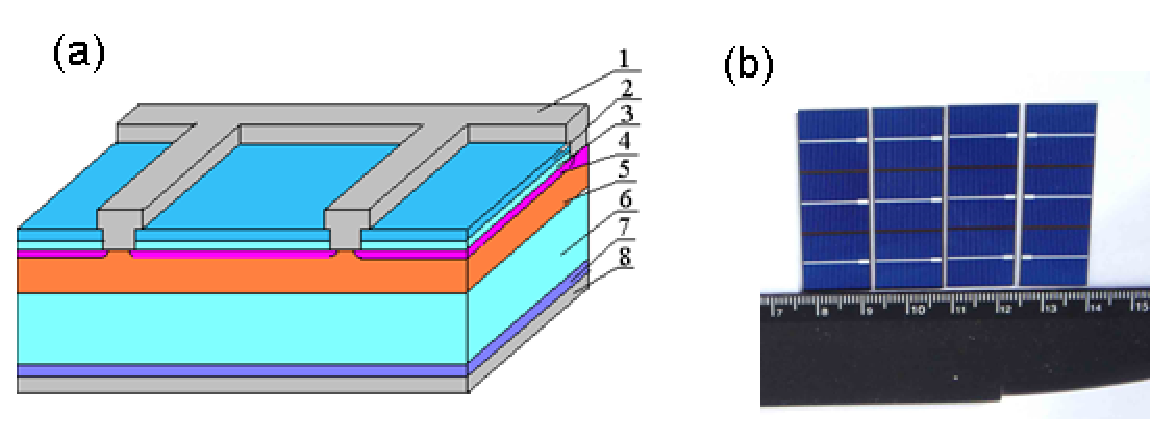
\includegraphics[width=0.5\textwidth]{Fig1}% Here is how to import EPS art
\caption{\label{Fig:sample}
(a) Scheme of the sample.
1 –-- frontal Al electrode;
2 –-- Si$_3$N$_4$;
3 –-- SiO$_2$;
4 –-- induced $n^{++}$-layer;
5 –-- diffusion $n^+$-layer;
6 –-- $p$-base region;
7 –-- diffusion $p^+$-layer;
8 –-- rear Al electrode.
(b) View of real solar cells;
the photo was taken from the side of frontal metal electrode.
}
\end{figure}

To dissociate FeB pairs, the frontal side of the sample was illuminated with a halogen lamp with radiation intensity $W_\mathrm{ill}$ of $0.08-0.20$~W/cm$^2$.
The illumination time $t_\mathrm{ill}$ \textcolor[rgb]{0.00,0.07,1.00}{\uline{was}} up to 30~s.


The FeB pair association was monitored by $t_\mathrm{ill}$ \textcolor[rgb]{0.00,0.07,1.00}{\uline{measuring}} the kinetics of
short circuit current $I_\mathrm{SC}(t)$ after halogen lamp illumination –-- see Fig.~\ref{Fig:Method}.
$I_\mathrm{SC}$ was measured under SC illumination by a low--intensity monochromatic light source (light--emitting diode SN--HPIR940nm--1W with light wavelength $\lambda=940$~nm).
\textcolor[rgb]{0.00,0.07,1.00}{\uline{
The excess carrier density $\Delta n$ induced by the LED illumination
was estimated by using open-circuit voltage value according to Sachenko \emph{et. al.}\cite{JAPSach}.
The $\Delta n$ value ($<10^{12}$ cm$^{-3}$) and duty cycle while $I_\mathrm{SC}(t)$ measuring (0.5\%)
evidence that LED illumination is weak and does not cause FeB dissociation.
After  illumination by the halogen lamp is terminated,
FeB pairs are formed again}}
and the starting value of $I_\mathrm{SC}$ is completely recovered.


\begin{figure}
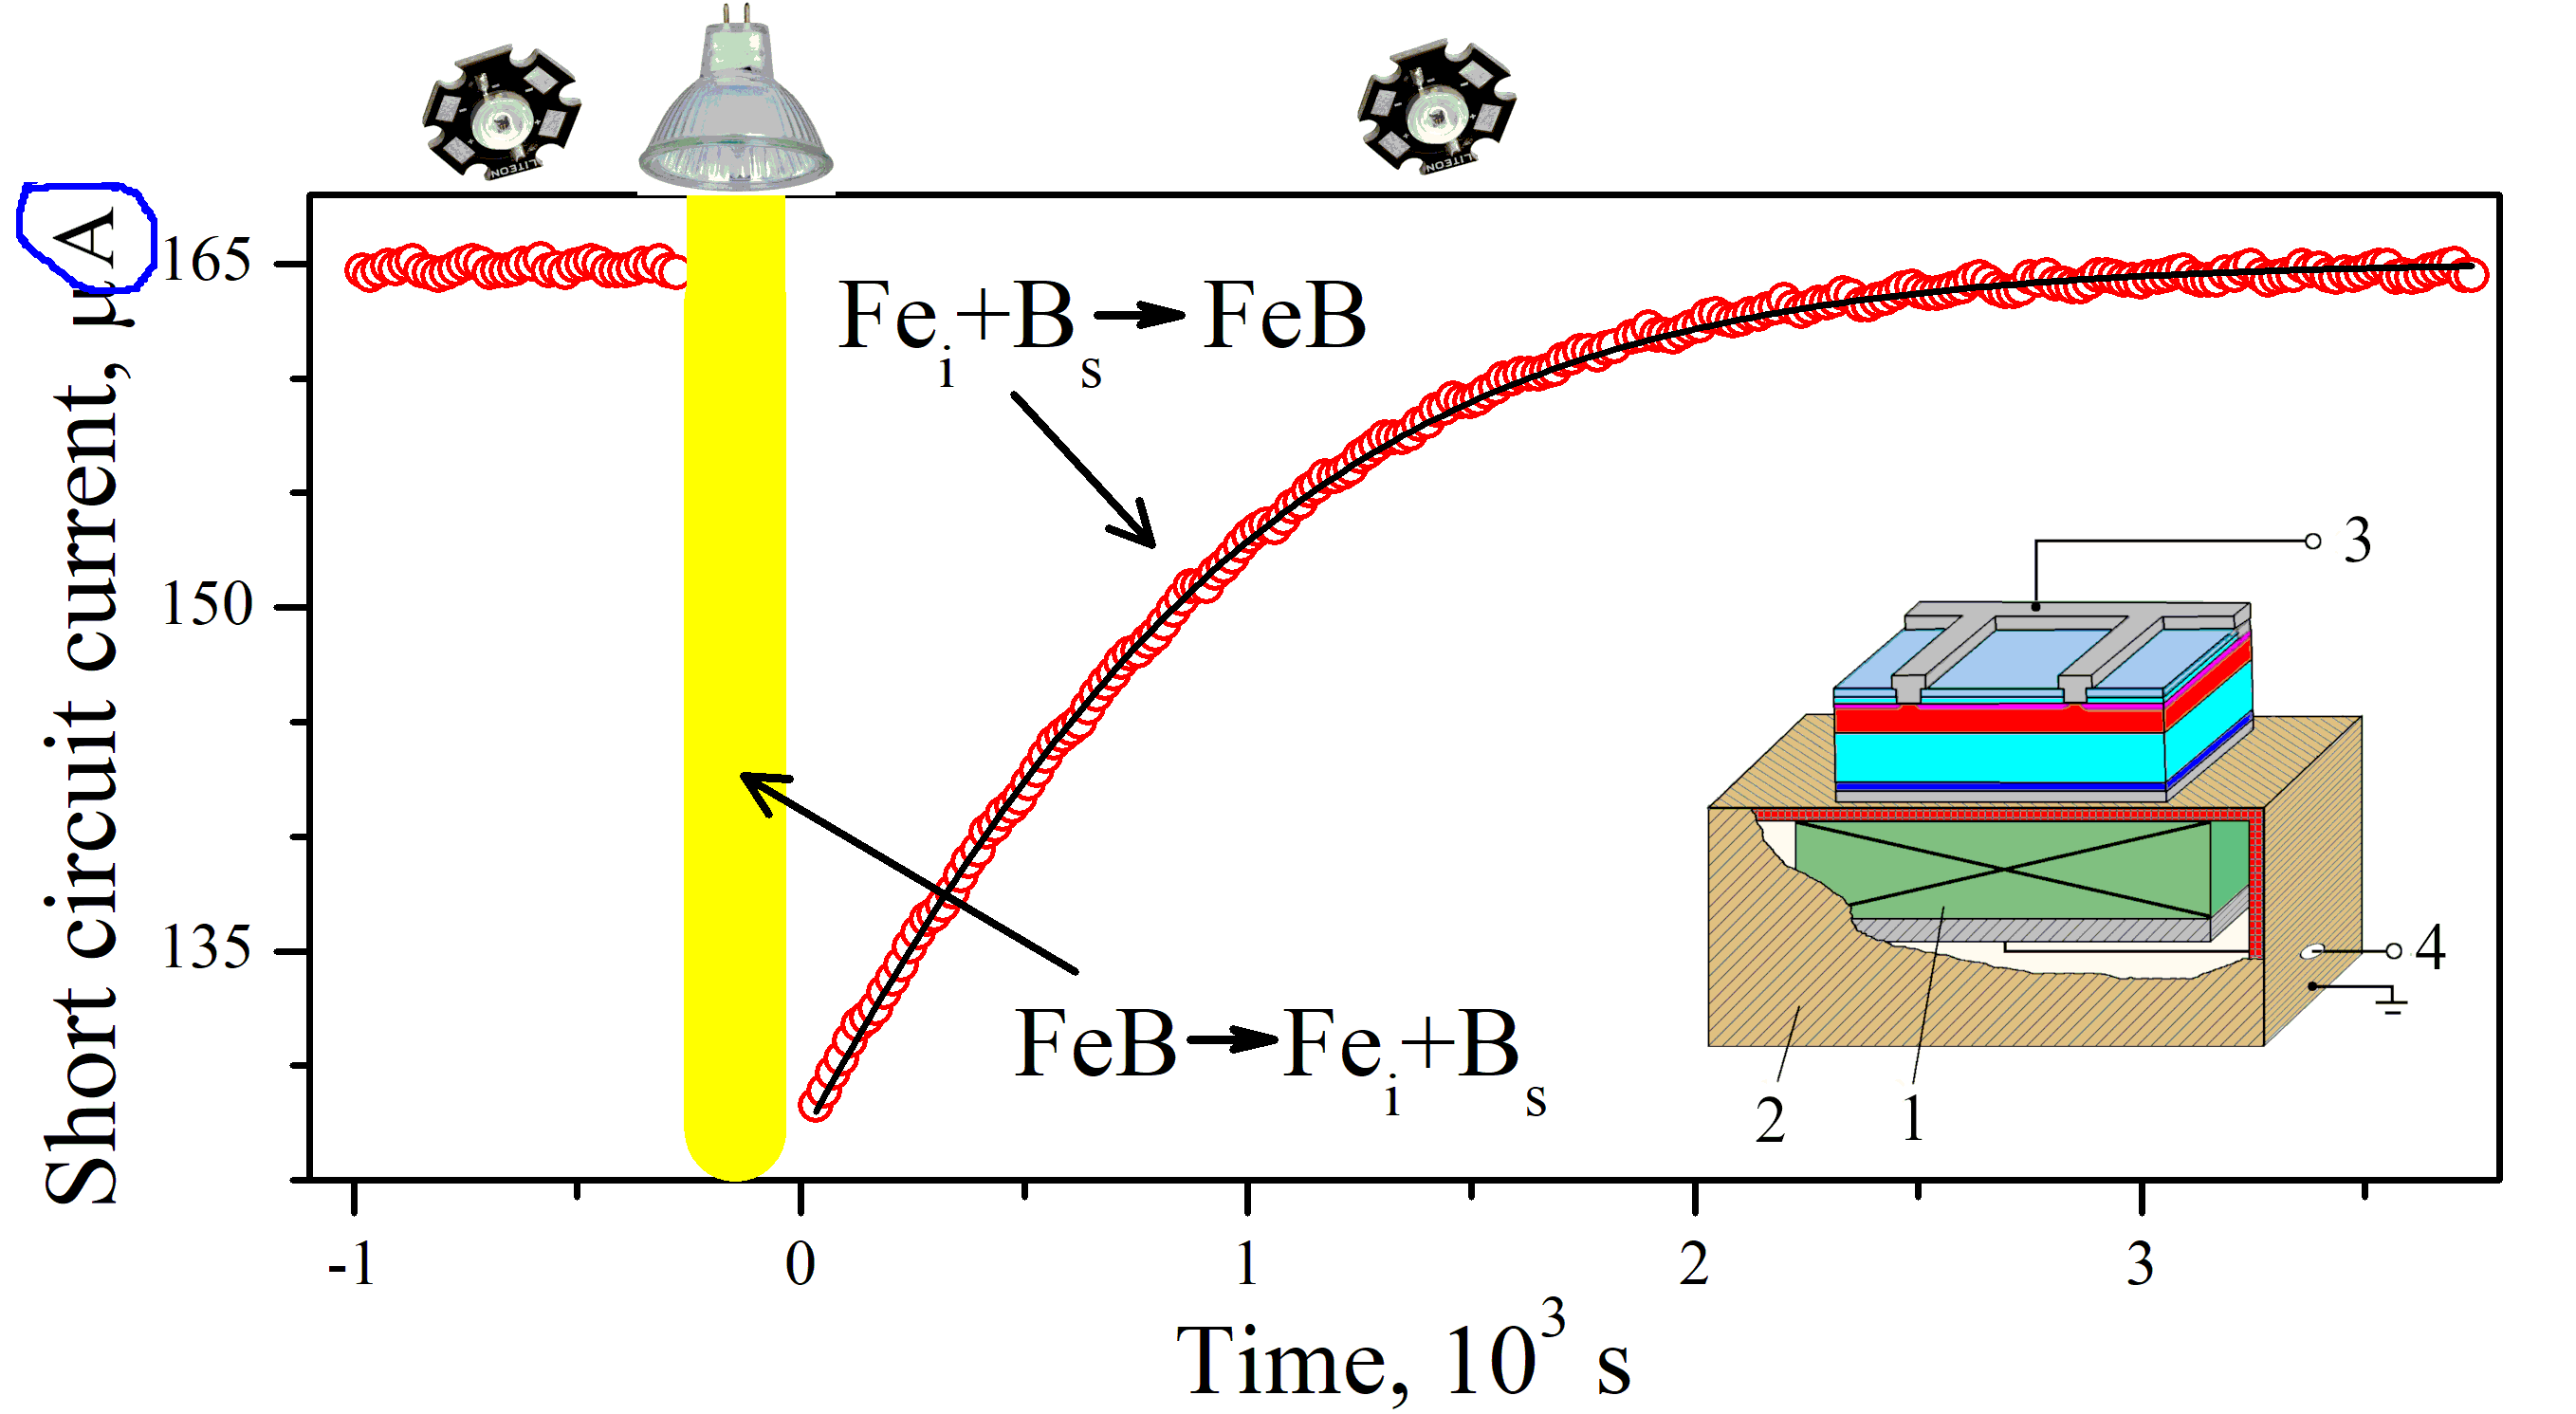
\includegraphics[width=0.5\textwidth]{Fig2}% Here is how to import EPS art
\caption{\label{Fig:Method}
Kinetics of short circuit current after intensive illumination.
The marks are the experimental results,
the line is the fitted curve using Eqs.~(\ref{eqIsc})-(\ref{eqNFeBt}).
The zero of time corresponds to the moment of intensive illumination termination.
$T=340$~K.
Inset: Scheme of USL.
1 –-- piezoelectric transducer;
2 –-- metal (Cu) foil ,
3 and 4 --- contact to $I$-–$V$ measure and to ultrasound excitation, respectively.
}
\end{figure}

In fact, in conditions of homogeneous carrier generation in the base, which is several minority carrier diffusion lengths $L_n$,
the short circuit current can be described as following \cite{Bube,Razeghi}:
\begin{equation}
\label{eqIsc}
I_\mathrm{SC}(t)=\frac{P_{ph}(1-R_{ph})\,q\beta\lambda}{hc}\cdot
\frac{\alpha_{ph}\sqrt{\mu_n k T \tau(t)/q}}{1+\alpha_{ph}\sqrt{\mu_n k T \tau(t)/q}}\,,
\end{equation}
where
$\alpha_{ph}=\alpha_{ph}(T,\lambda)$ is the coefficient of light absorption,
$P_{ph}$ is the light power,
$R_{ph}$ is the coefficient of reflection,
$\beta$ is the coefficient of quantum  yield,
$\mu_n$ is the electron mobility,
$\tau$ is the minority carrier lifetime in the base.
In the assumption that it is the iron--related defects that play an essential role in the recombination, the following expression can be used to estimate $\tau$:
\begin{equation}
\label{eqTau}
\frac{1}{\tau(t)}=\frac{1}{\tau_i}+\frac{1}{\tau_{SRH}^{\mathrm{Fe_i}}(t)}
+\frac{1}{\tau_{SRH}^\mathrm{FeB}(t)}+\frac{1}{\tau_{other}}\,,
\end{equation}
where
$\tau_i$ is the lifetime associated with intrinsic recombination,
$\tau_{SRH}^{\mathrm{Fe_i}}$ and $\tau_{SRH}^\mathrm{FeB}$ are related to the recombinations at interstitial iron atoms Fe$_i$ and at FeB pairs, accordingly;
$\tau_{other}$ describes further recombination channels
(other impurities, lattice defects, surface recombination).
In order to calculate $\tau_{SRH}^{\mathrm{Fe_i}}$ and $\tau_{SRH}^\mathrm{FeB}$
Shockley--Read--Hall model was used
%\begin{equation}
%\label{eqTauSRH}
%\tau_{SRH}^\mathrm{Fe_i,FeB}(t)=\frac{\tau_{p0}^\mathrm{Fe_i,FeB}(t)\cdot(n_0+n_1+\Delta n)
%+\tau_{n0}(t)\cdot(N_A+p_1+\Delta n)}
%{N_A+n_0+\Delta n}\,,
%\end{equation}
\begin{eqnarray}
\label{eqTauSRH}
\tau_{SRH}^\mathrm{Fe_i,FeB}(t)=\frac{\tau_{p0}^\mathrm{Fe_i,FeB}(t)
\cdot(n_0+n_1^\mathrm{Fe_i,FeB}+\Delta n)}
{N_A+n_0+\Delta n}+\nonumber\\
\frac{\tau_{n0}^\mathrm{Fe_i,FeB}(t)\cdot(N_A+p_1^\mathrm{Fe_i,FeB}+\Delta n)}
{N_A+n_0+\Delta n}\,,
\end{eqnarray}
where
$N_A$ is the material’s doping level  \textcolor[rgb]{0.00,0.07,1.00}{\uline{($1.4\cdot10^{15}$~cm$^{-3}$)}},
$n_0$ is the equilibrium electron concentration given by the law of mass action;
$n_1$ and $p_1$ are given by
%\begin{equation}
%\label{eqp1n1}
%n_1^\mathrm{Fe_i,FeB}=N_C \exp\left(-\frac{E_C-E_t^\mathrm{Fe_i,FeB}}{kT}\right), \quad
%p_1^\mathrm{Fe_i,FeB}=N_V \exp\left(-\frac{E_t^\mathrm{Fe_i,FeB}-E_V}{kT}\right)\,,
%\end{equation}
\begin{eqnarray}
\label{eqp1n1}
n_1^\mathrm{Fe_i,FeB}=N_C \exp\left(-\frac{E_C-E_t^\mathrm{Fe_i,FeB}}{kT}\right)\,,\nonumber\\
p_1^\mathrm{Fe_i,FeB}=N_V \exp\left(-\frac{E_t^\mathrm{Fe_i,FeB}-E_V}{kT}\right)\,,
\end{eqnarray}
where
$E_C$ and $E_V$ are the energies of the conduction band and valence band edge, respectively,
$N_C$ and $N_V$ are the densities of states in the conduction band and valence band, respectively, and $E_t$ is the energy level of the relevant defect.
The respective capture time constants of electrons and holes at the defect are given by
\begin{eqnarray}
\label{eqtaupn}
\tau_{p0}^\mathrm{Fe_i,FeB}(t)=\frac{1}{N_\mathrm{Fe,FeB}(t)\sigma_p^\mathrm{Fe_i,FeB}\upsilon_{th}^p}\,,\nonumber\\
\tau_{n0}^\mathrm{Fe_i,FeB}(t)=\frac{1}{N_\mathrm{Fe,FeB}(t)\sigma_n^\mathrm{Fe_i,FeB}\upsilon_{th}^n}\,,
\end{eqnarray}
where
$N_\mathrm{Fe}(t)$ and $N_\mathrm{FeB}(t)$ are the concentration of Fe$_i$ and FeB, respectively,
$\upsilon_{th}$ is the thermal velocity,
and $\sigma_n$ and $\sigma_p$ are the respective capture cross-sections of electrons and holes at the defect.

The time dependence of interstitial iron atom concentration after pair dissociation is described by the known expression from \cite{MurphyJAP2011,FeB:kinetic}:
\begin{equation}
\label{eqNFet}
N_\mathrm{Fe}(t)=(N_\mathrm{Fe,0}-N_\mathrm{Fe,eq})\cdot
\exp(-t/\tau_\mathrm{ass})+N_\mathrm{Fe,eq}\,,
\end{equation}
where
$\tau_\mathrm{ass}$ is the characteristic time of the complex association,
according to \cite{FeBKin2019,FeBAssJAP2014,FeBAssSST2011}
\begin{equation}
\label{eqTass}
\tau_\mathrm{ass}=5.7\cdot10^5\,\textcolor[rgb]{0.00,0.07,1.00}{\uline{\frac{\mathrm{s}}{\mathrm{K}\cdot\mathrm{cm}^3}}}\cdot\frac{T}{N_A}\exp\left(\frac{E_m}{kT}\right)\,,
\end{equation}
where $E_m$ is the energy of Fe$_i^+$ migration;
$N_\mathrm{Fe,0}$ is the concentration of interstitial iron atoms formed due to illumination and $N_\mathrm{Fe,eq}$ is the portion of  interstitial iron atoms with $N_\mathrm{Fe,0}$  that remain unpaired in equilibrium state.
According to Wijaranakula\cite{FeB:kinetic},
$N_\mathrm{Fe,eq}$ depends on temperature, doping level and $N_\mathrm{Fe,0}$:
$N_\mathrm{Fe,eq}= N_\mathrm{Fe,eq}(T, N_A, N_\mathrm{Fe,0})$.
The estimations show that  at 340~K  $N_\mathrm{Fe,eq}\simeq0.1 N_\mathrm{Fe,0}$
for the samples under study.

In its turn, the iron--boron pair concentration $N_\mathrm{FeB}$, which is formed in the result of the partial association of $N_\mathrm{Fe,0}$ can be estimated from
\begin{equation}
\label{eqNFeBt}
N_\mathrm{FeB}(t)+N_\mathrm{Fe}(t)=N_\mathrm{Fe,0}\,.
\end{equation}
In case the intensive illumination causes dissociation of all the pairs,
$N_\mathrm{Fe,0}$ should be the same as the total concentration of the impurity iron in the structure $N_\mathrm{Fe,tot}$.
If the duration (or intensity) of illumination is not sufficient for total dissociation,
$N_\mathrm{Fe,0}< N_\mathrm{Fe,tot}$.
In the latter case $\tau_{other}$ will also make contribution in the
recombination of the FeB pairs that have not dissociated
(with concentration $N_\mathrm{Fe,tot}-N_\mathrm{Fe,0}-N_\mathrm{Fe,eq}(T, N_A, N_\mathrm{Fe,tot}-N_\mathrm{Fe,0})$)
as well as the respective number of Fe$_i$
(with concentration $N_\mathrm{Fe,eq}(T, N_A, N_\mathrm{Fe,tot}-N_\mathrm{Fe,0})$).

In our calculations,
we took $\beta=1$,
$R_{ph}=0.14$ (the result of calculations  according to Klyui \emph{et al.}\cite{KostRefl2000}),
$\mu_n(T, N_A)$ from Klaassen \cite{KLAASSEN953},
$\upsilon_{th}^n$ and $\upsilon_{th}^p$ from Green\cite{Nc:Green},
$N_C$, $N_V$ from Couderc \emph{et al.}\cite{Si_ni_Couderc},
the defect parameters from Rougieux \emph{et al.}\cite{ROUGIEUX2018},
$\alpha_{ph} (T,\lambda)$ from data\cite{Si:Absorb,GreenOptic}.
In calculating $\tau_i$, band--to--band radiation recombination and Auger recombination were taken into account,
and the temperature dependence of the corresponding coefficients
was calculated according to Nguyen \emph{et al.}\cite{Si_BtB} and Altermatt \emph{et al.}\cite{Si_Auger}.
We used Eqs.~(\ref{eqIsc})-(\ref{eqNFeBt}) to fit the experimental data $I_\mathrm{SC}(t)$.
As fitting parameters  $P_{ph}$, $\tau_{other}$, $N_\mathrm{Fe,0}$, and $E_m$  were taken.
The fittings were performed by using the metaheuristic method EBLSHADE \cite{EBLSHADE}.

The example of fitting results is shown in Fig.~\ref{Fig:Method}.
In our case, the parameters determined by fitting had the following values.
$P_{ph} = (3.6\pm0.2)\cdot10^{-4}$~W which agrees well
with the value measured by PowerMeter Rk-5720 ($3.5\cdot10^{-4}$~W).
$\tau_{other}>100$~s, which testifies that the contribution of other recombination pathways can be neglected.
$N_\mathrm{Fe,0}=(1.6\pm0.1)\cdot10^{13}$~cm$^{-3}$,
which is close to the value obtained for the samples of the same series from $L_n$ measuring before and after illumination ($0.5\cdot10^{13}$~cm$^{-3}$).
\textcolor[rgb]{0.00,0.07,1.00}{\uline{
In this case $L_{n}$ was measured using spectral dependencies of short circuit current\cite{LnIscMethod},
the iron concentration was determined by using Zoth and Bergholz\cite{FeB_Zong} equation.}}
Finally, $E_m = (0.655\pm0.001)$~eV.
This value coincides with that well known \cite{FeBAssJAP2014,FeBkinAPL2008,FeBKin2019,FeBAssSST2011} which is $0.66$~eV.
The coincidence of the values obtained by approximation
with those obtained from other sources (first of all, $E_m$ value) proves
that the investigations of $I_\mathrm{SC}(t)$ after intensive illumination can be applied
\textcolor[rgb]{0.00,0.07,1.00}{\uline{for estimating}} the parameters of iron-related defects.
Moreover, the peculiarities of pair dissociation (see Sec.~\ref{sec:FeBdis}) found in this way also correspond to those reported in the previous publications, which testifies that this approach is quite appropriate.
In fact, the time of $I_\mathrm{SC}$ recovering is an indicator of how large \textcolor[rgb]{0.00,0.07,1.00}{\uline{the energy of migration is}},
and the amplitude with which $I_\mathrm{SC}$ changes in the result of intensive illumination is associated with the concentration of iron atoms released in the process.
It should be also noted that this approach is similar to the method proposed
by Herlufsen \emph{et al.}\cite{FeMethod2012}, in which actual concentrations of FeB pairs are estimated by the photoluminescence signal kinetics during pair association.

The measurements were carried out over a temperature range of $300-340$~K.
The temperature was varied by a thermoelectric cooler controlled by STS-21 sensor and stabilized by a computer-controlled PID loop.

In case of USL, the transverse (with frequency $f_\mathrm{US}=0.3$~MHz) or
longitudinal ($2-31$~MHz) acoustic waves (AWs) were applied to the samples by using a piezoelectric transducer.
The US intensities $W_\mathrm{US}$ and amplitudes of \textcolor[rgb]{0.00,0.07,1.00}{\uline{strain}}
$\xi_\mathrm{US}=\sqrt{2W_\mathrm{US}/\rho_\mathrm{Si}\vartheta_\mathrm{US}^3}$
($\rho_\mathrm{Si}=2.33$~g/cm$^3$ is the silicon density,
$\vartheta_\mathrm{US}$ is the US velocity, 9850~m/s and 5840~m/s in cases of longitudinal and transverse AWs, respectively)
does not overcome 1.3~W/cm$^2$ and $2\cdot10^{-6}$, respectively.
Since the focus of our research was the influence of elastic vibrations on  FeB pair transformations,   to avoid the effect of
\textcolor[rgb]{0.00,0.07,1.00}{\uline{the}} piezoelectric field, the transducer was shielded --– see inset in Fig.~\ref{Fig:Method}.




\section{\label{sec:Rez}Results and discussion}
\subsection{\label{sec:FeBdis}FeB dissociation}


In our investigation of light--induced FeB pair dissociation processes,
we illuminated the structure with a halogen lamp varying the time of illumination
$t_\mathrm{ill}$ and afterward measured the
kinetics of short circuit current recovery –-- see Fig.~\ref{Fig:IscKin}(a).
As seen from the figure, the time of short circuit current recovery does not change while the amplitude of light--induced changes depends on the time of illumination.
Further approximation of the experimental curves by using the approach described in the previous section allowed us to estimate the number of pairs that dissociated in the result of illumination $N_\mathrm{Fe,0}$ as a function of $t_\mathrm{ill}$.
The experiments were carried out on a series of samples
at different light intensities and temperatures in conditions with  and without US loading.
The typical results are given in Fig.~\ref{Fig:Nfe_till}.

\begin{figure*}
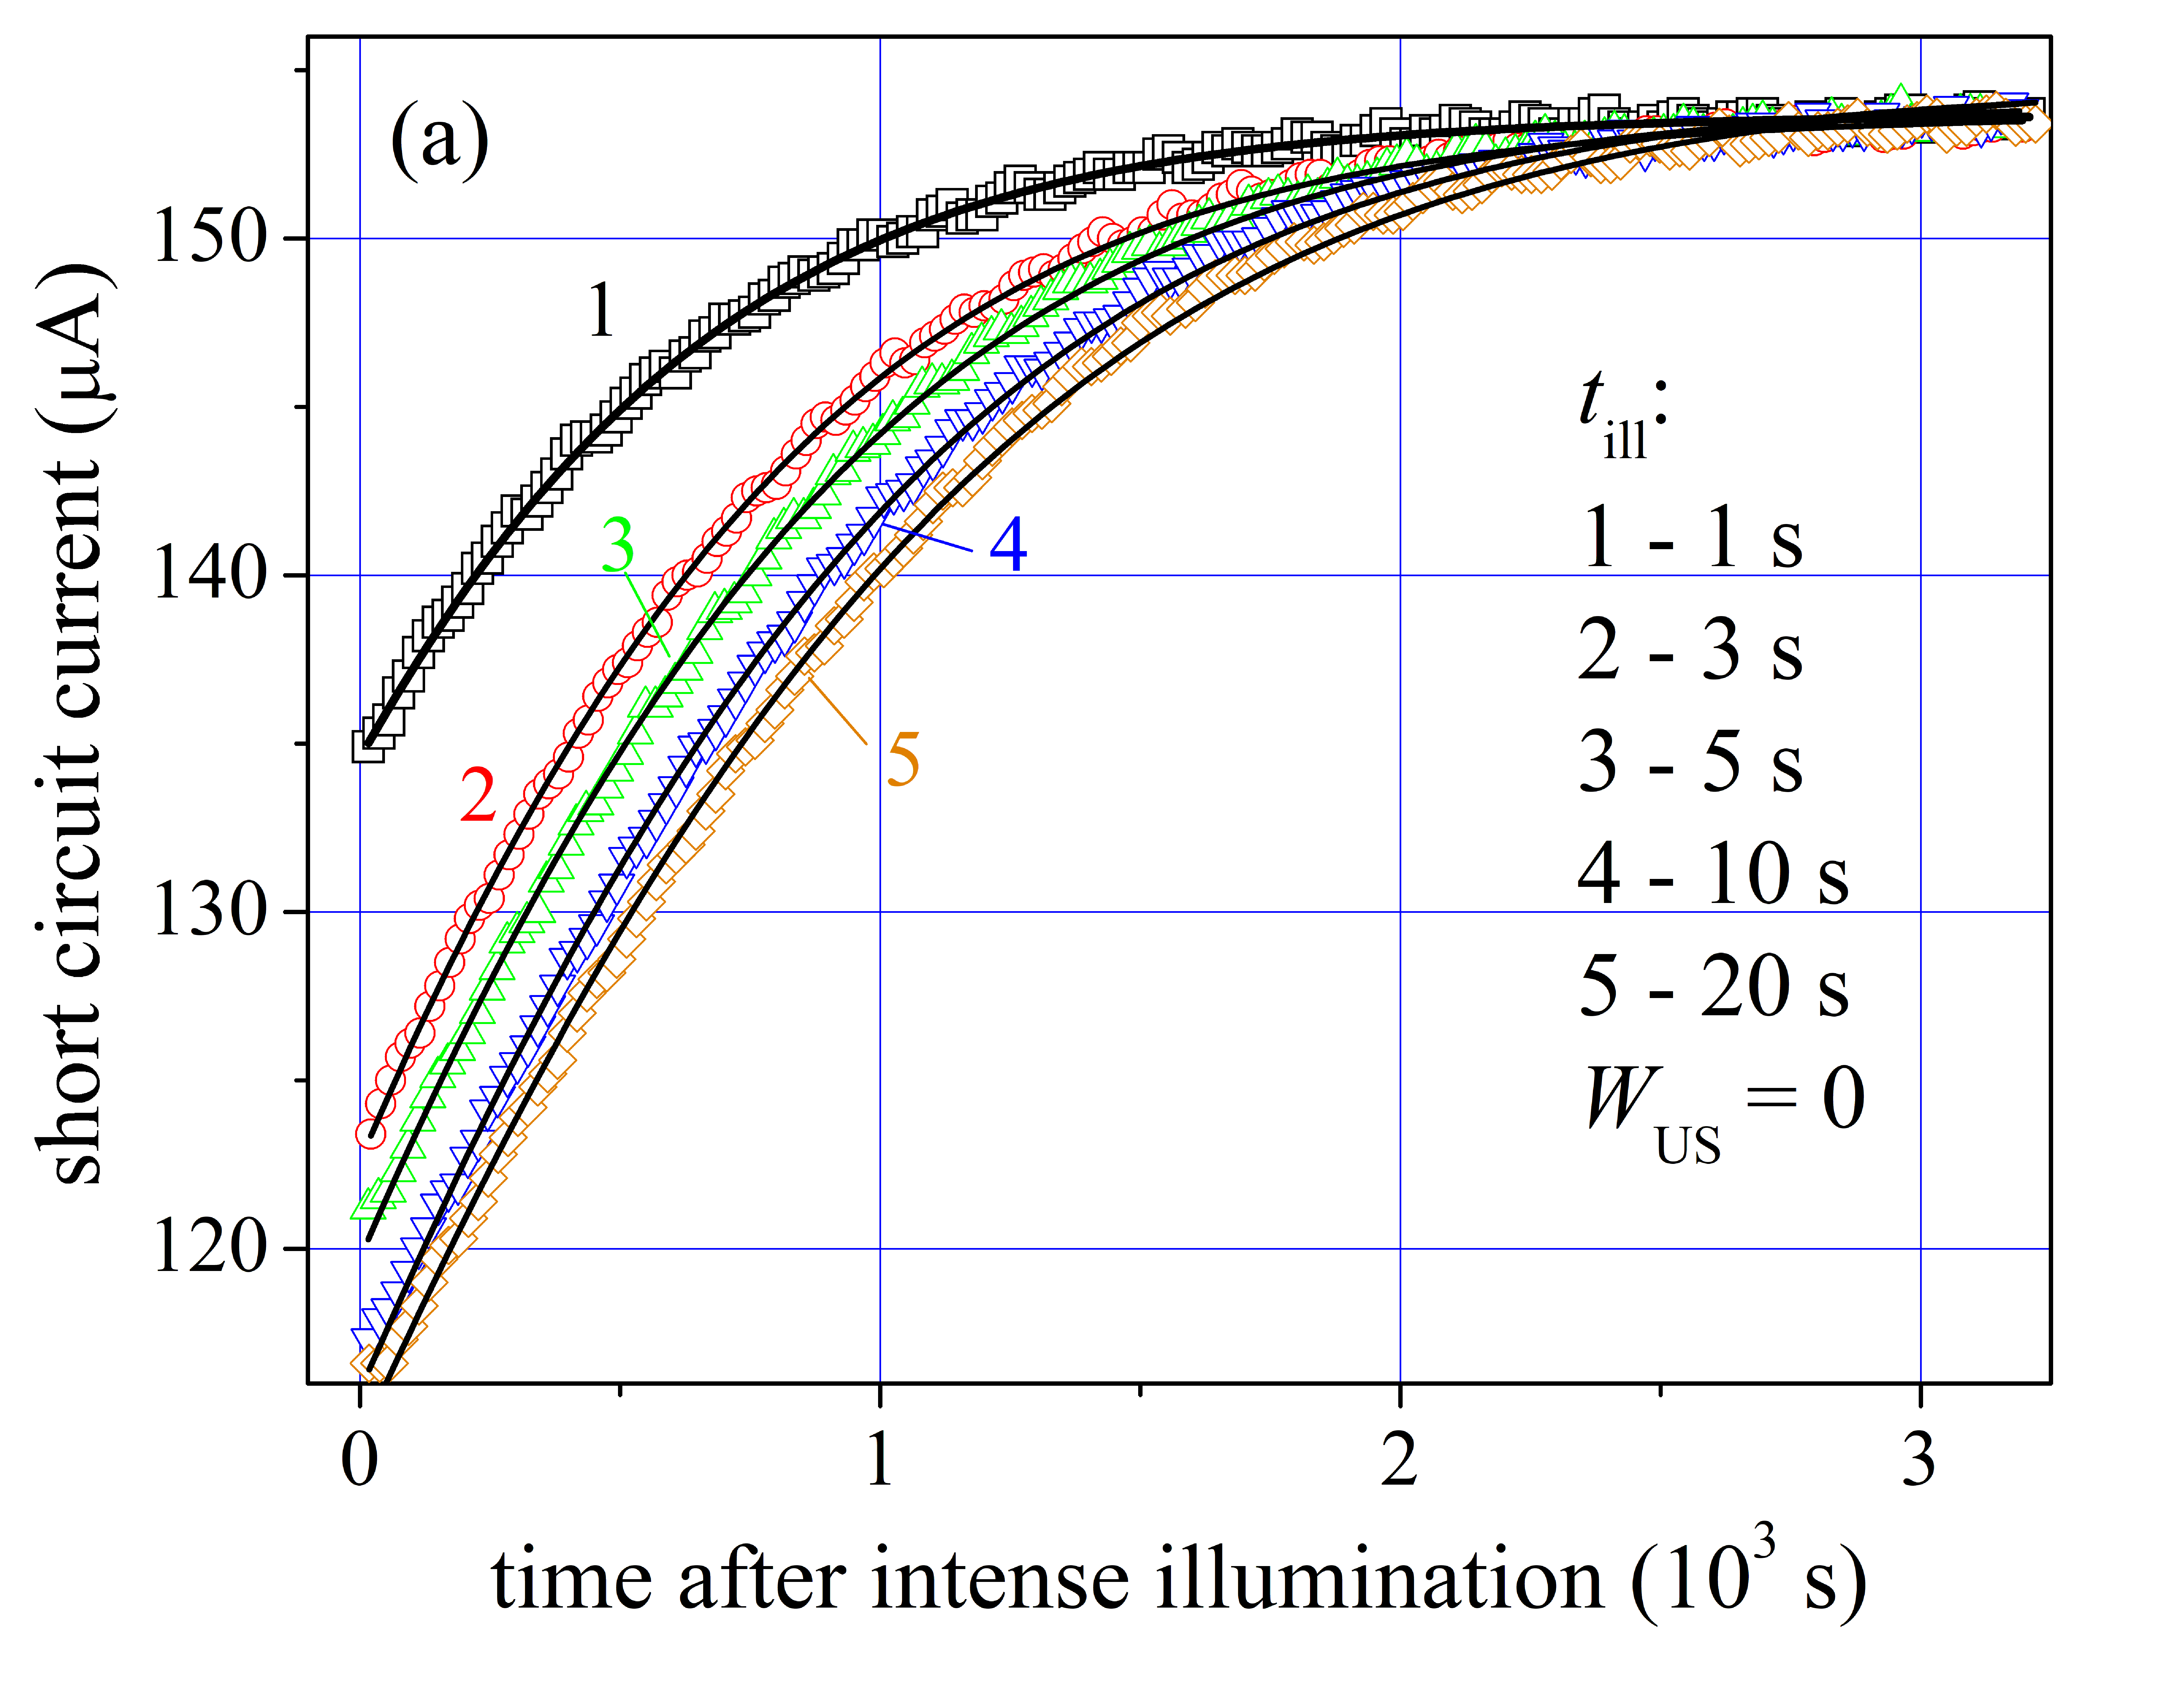
\includegraphics[width=0.45\textwidth]{Fig3a}% Here is how to import EPS art
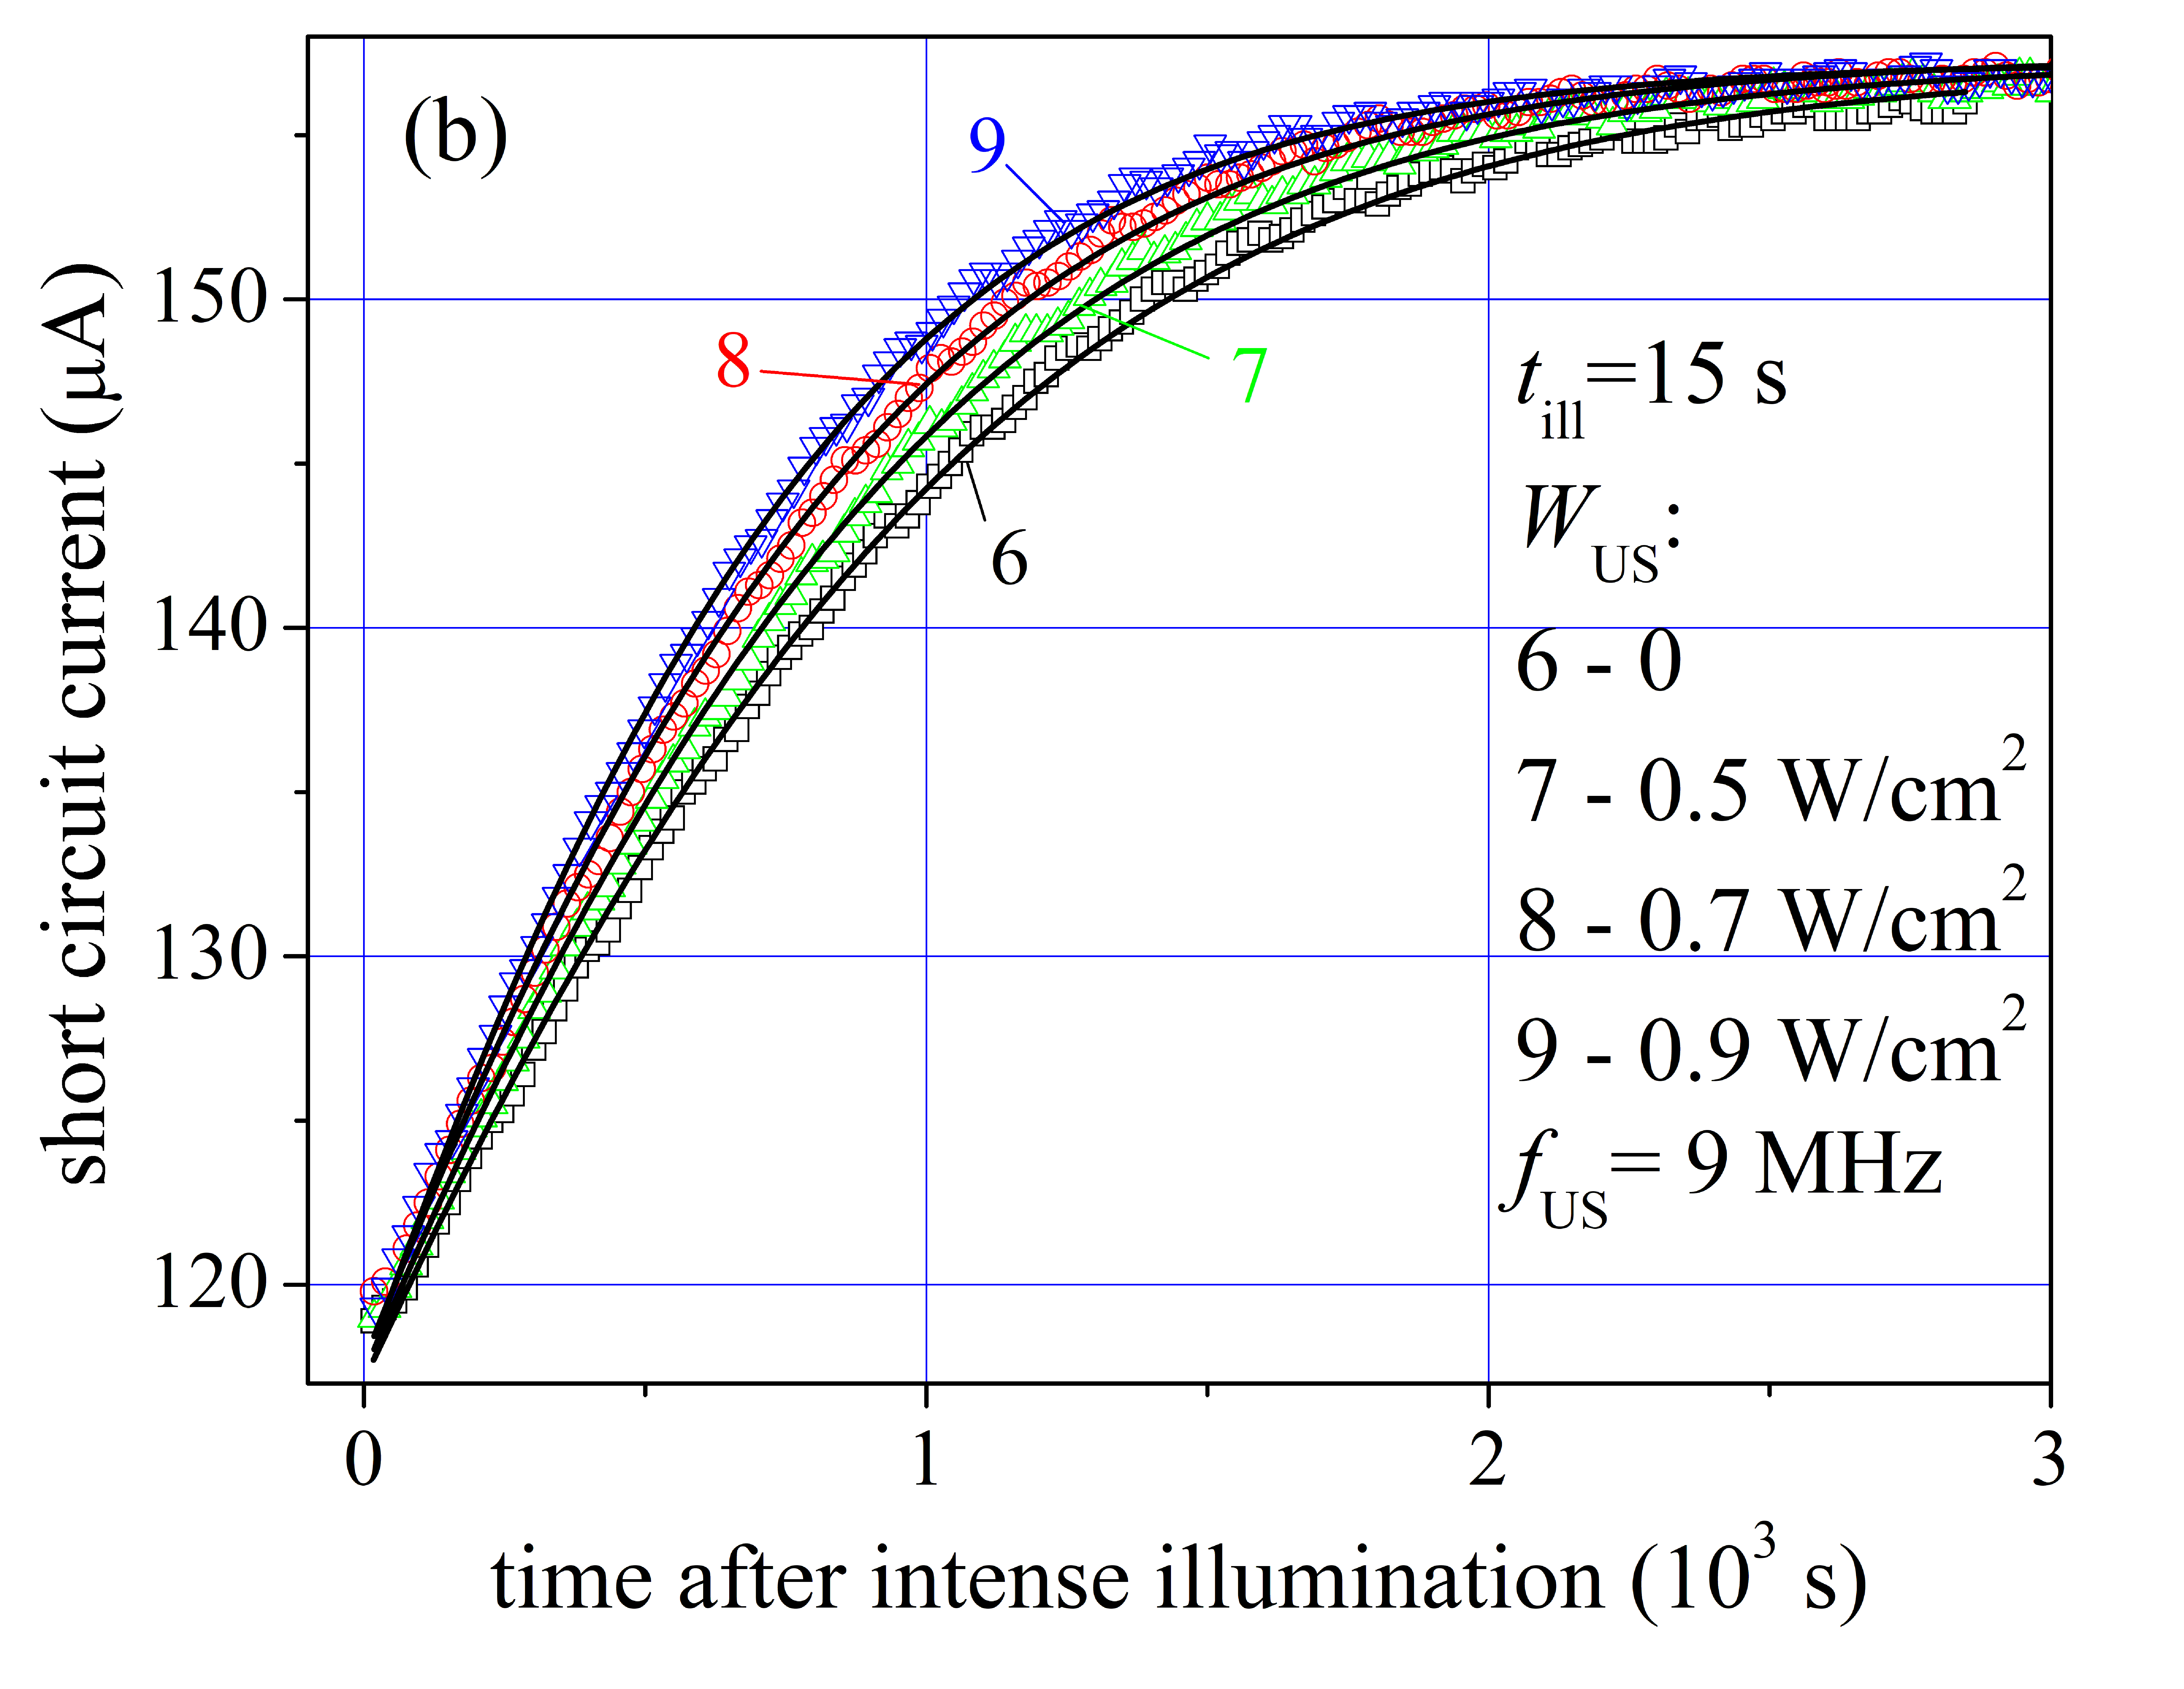
\includegraphics[width=0.45\textwidth]{Fig3b}% Here is how to import EPS art
\caption{\label{Fig:IscKin}
Typical kinetics of short circuit current after intensive illumination of different duration (a) and USL intensity (b). T
he marks are the experimental results,
the lines are the curves fitted by using Eqs.~(\ref{eqIsc})-(\ref{eqNFeBt}).
$t_\mathrm{ill}$, s: 1 (curve 1), 3 (2), 5 (3), 10 (4), 15 (6-9), 20 (5).
$W_\mathrm{US}$, W/cm$^2$: 0 (1-6), 0.5 (7), 0.7 (8), 0.9 (9).
$f_\mathrm{US}=9$~MHz, $T=340$~K.
}
\end{figure*}

\begin{figure*}
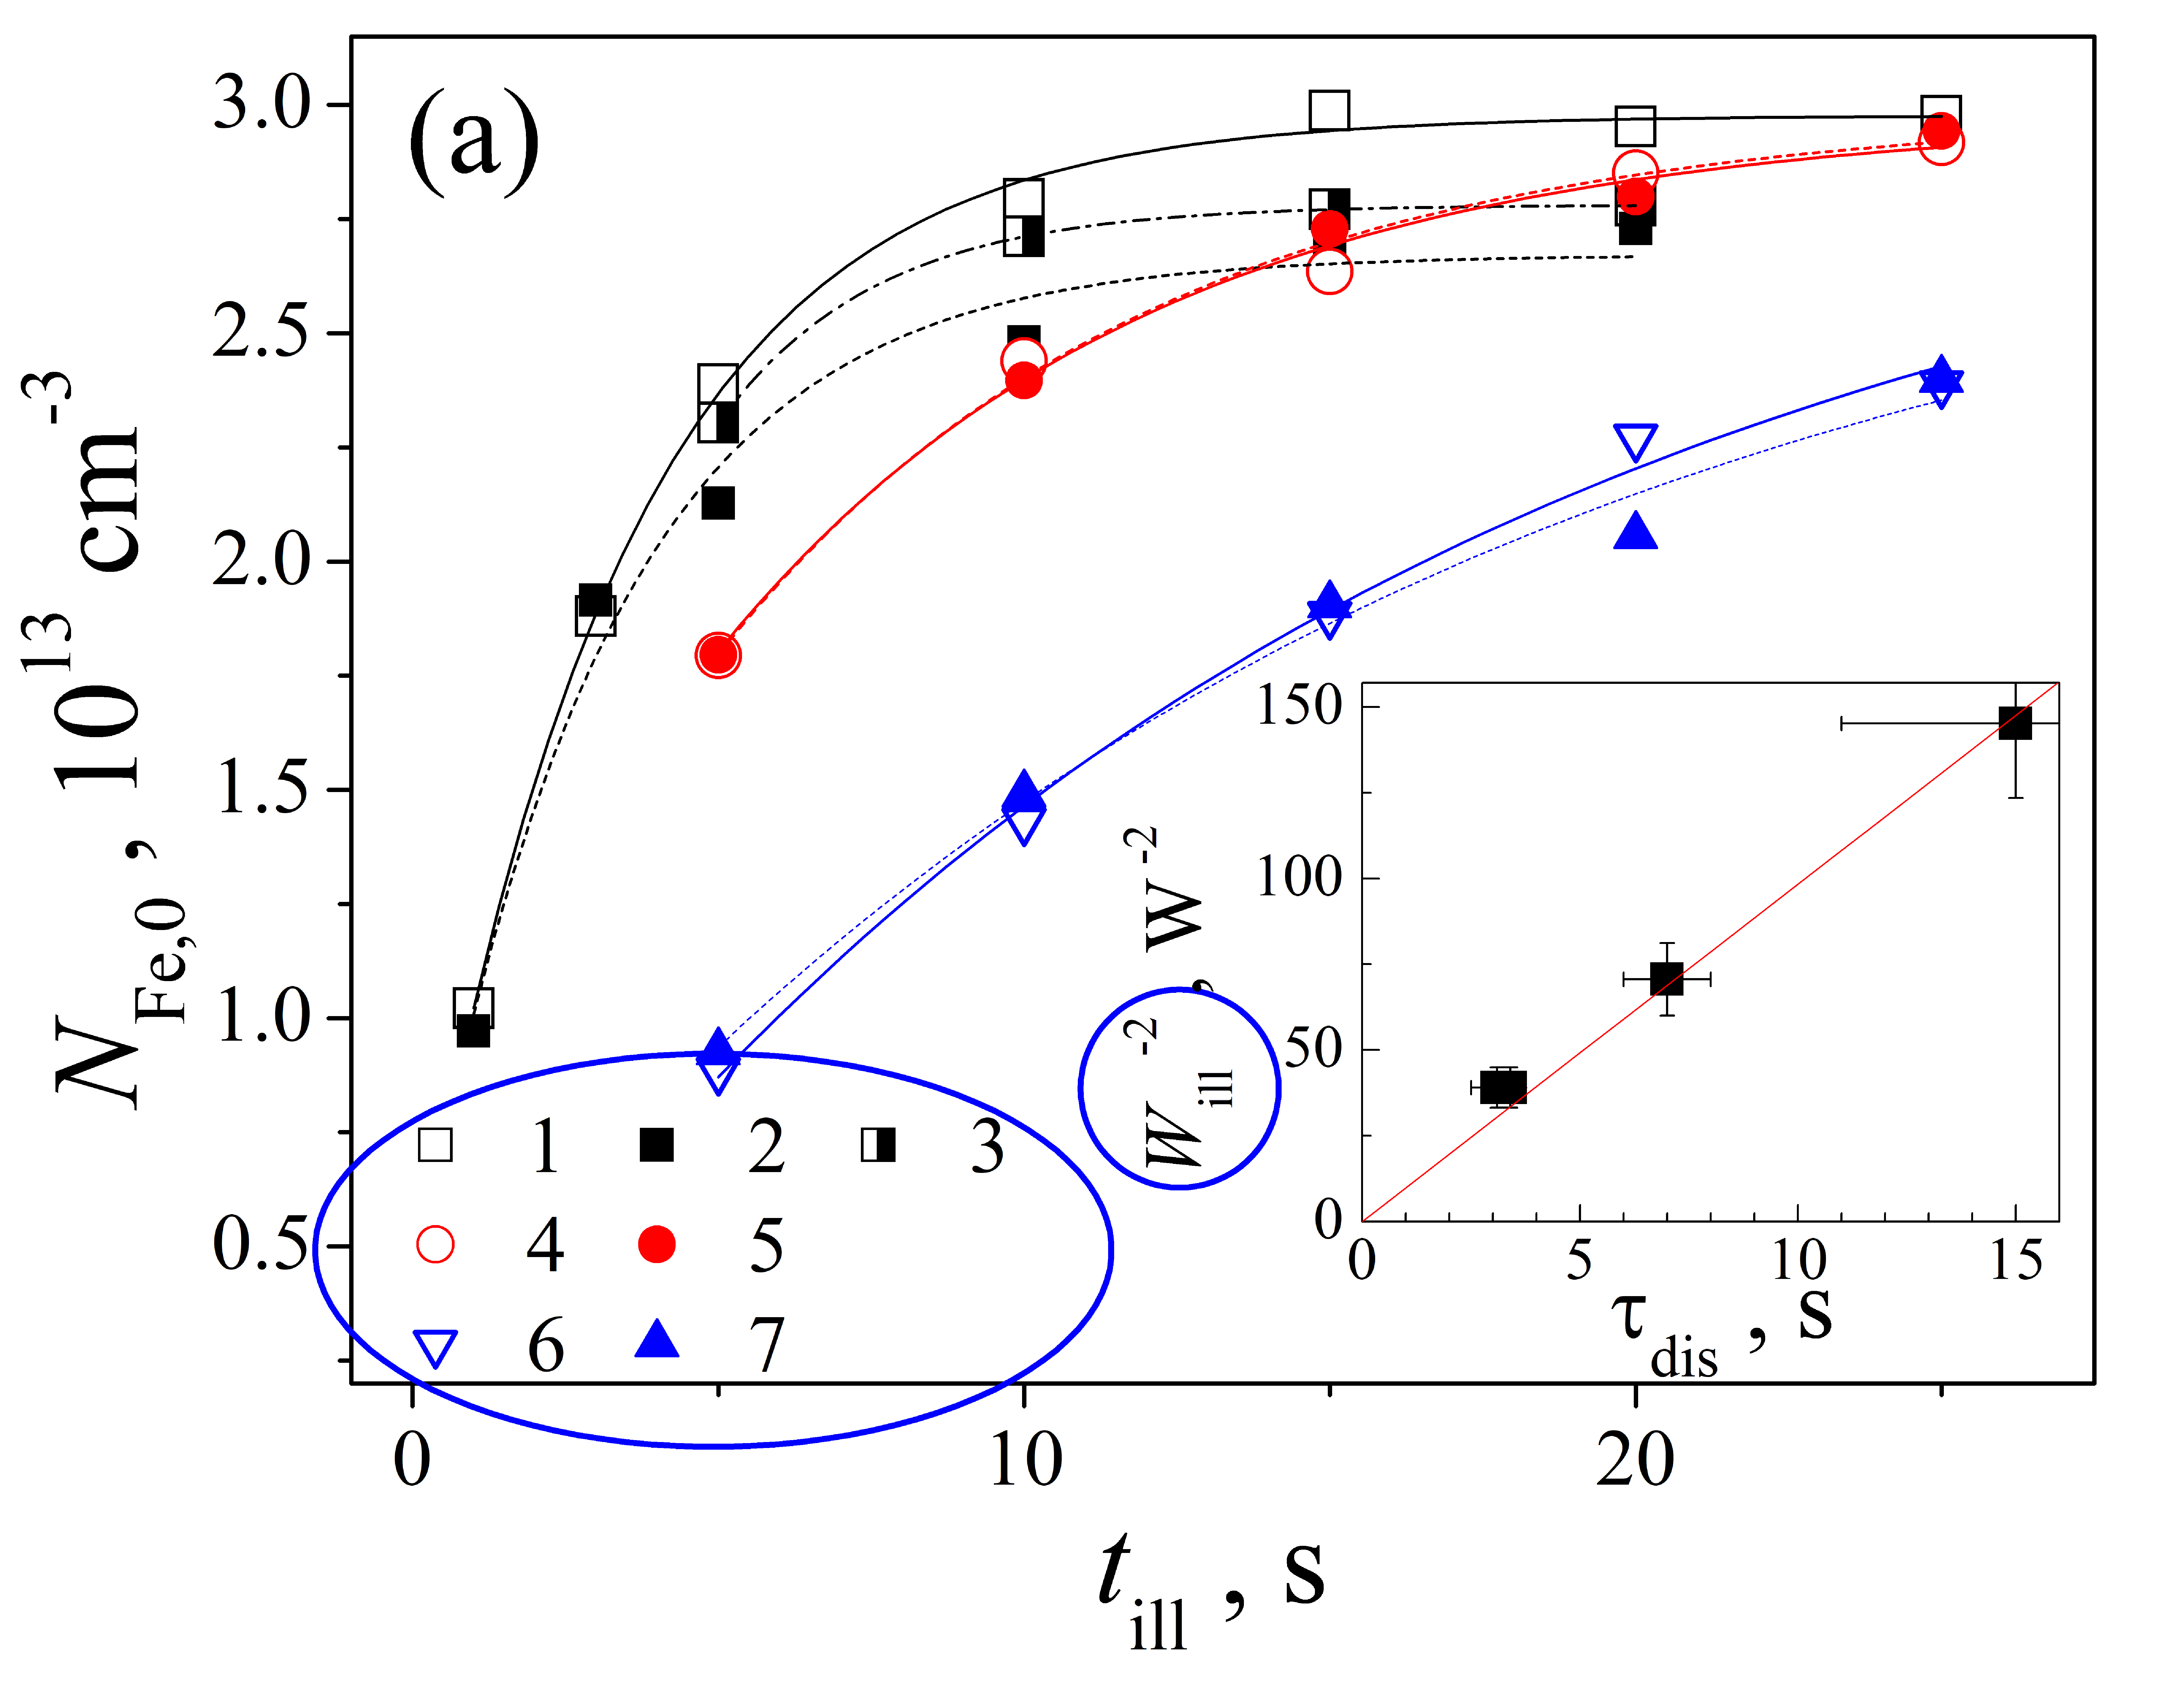
\includegraphics[width=0.33\textwidth]{Fig4a}% Here is how to import EPS art
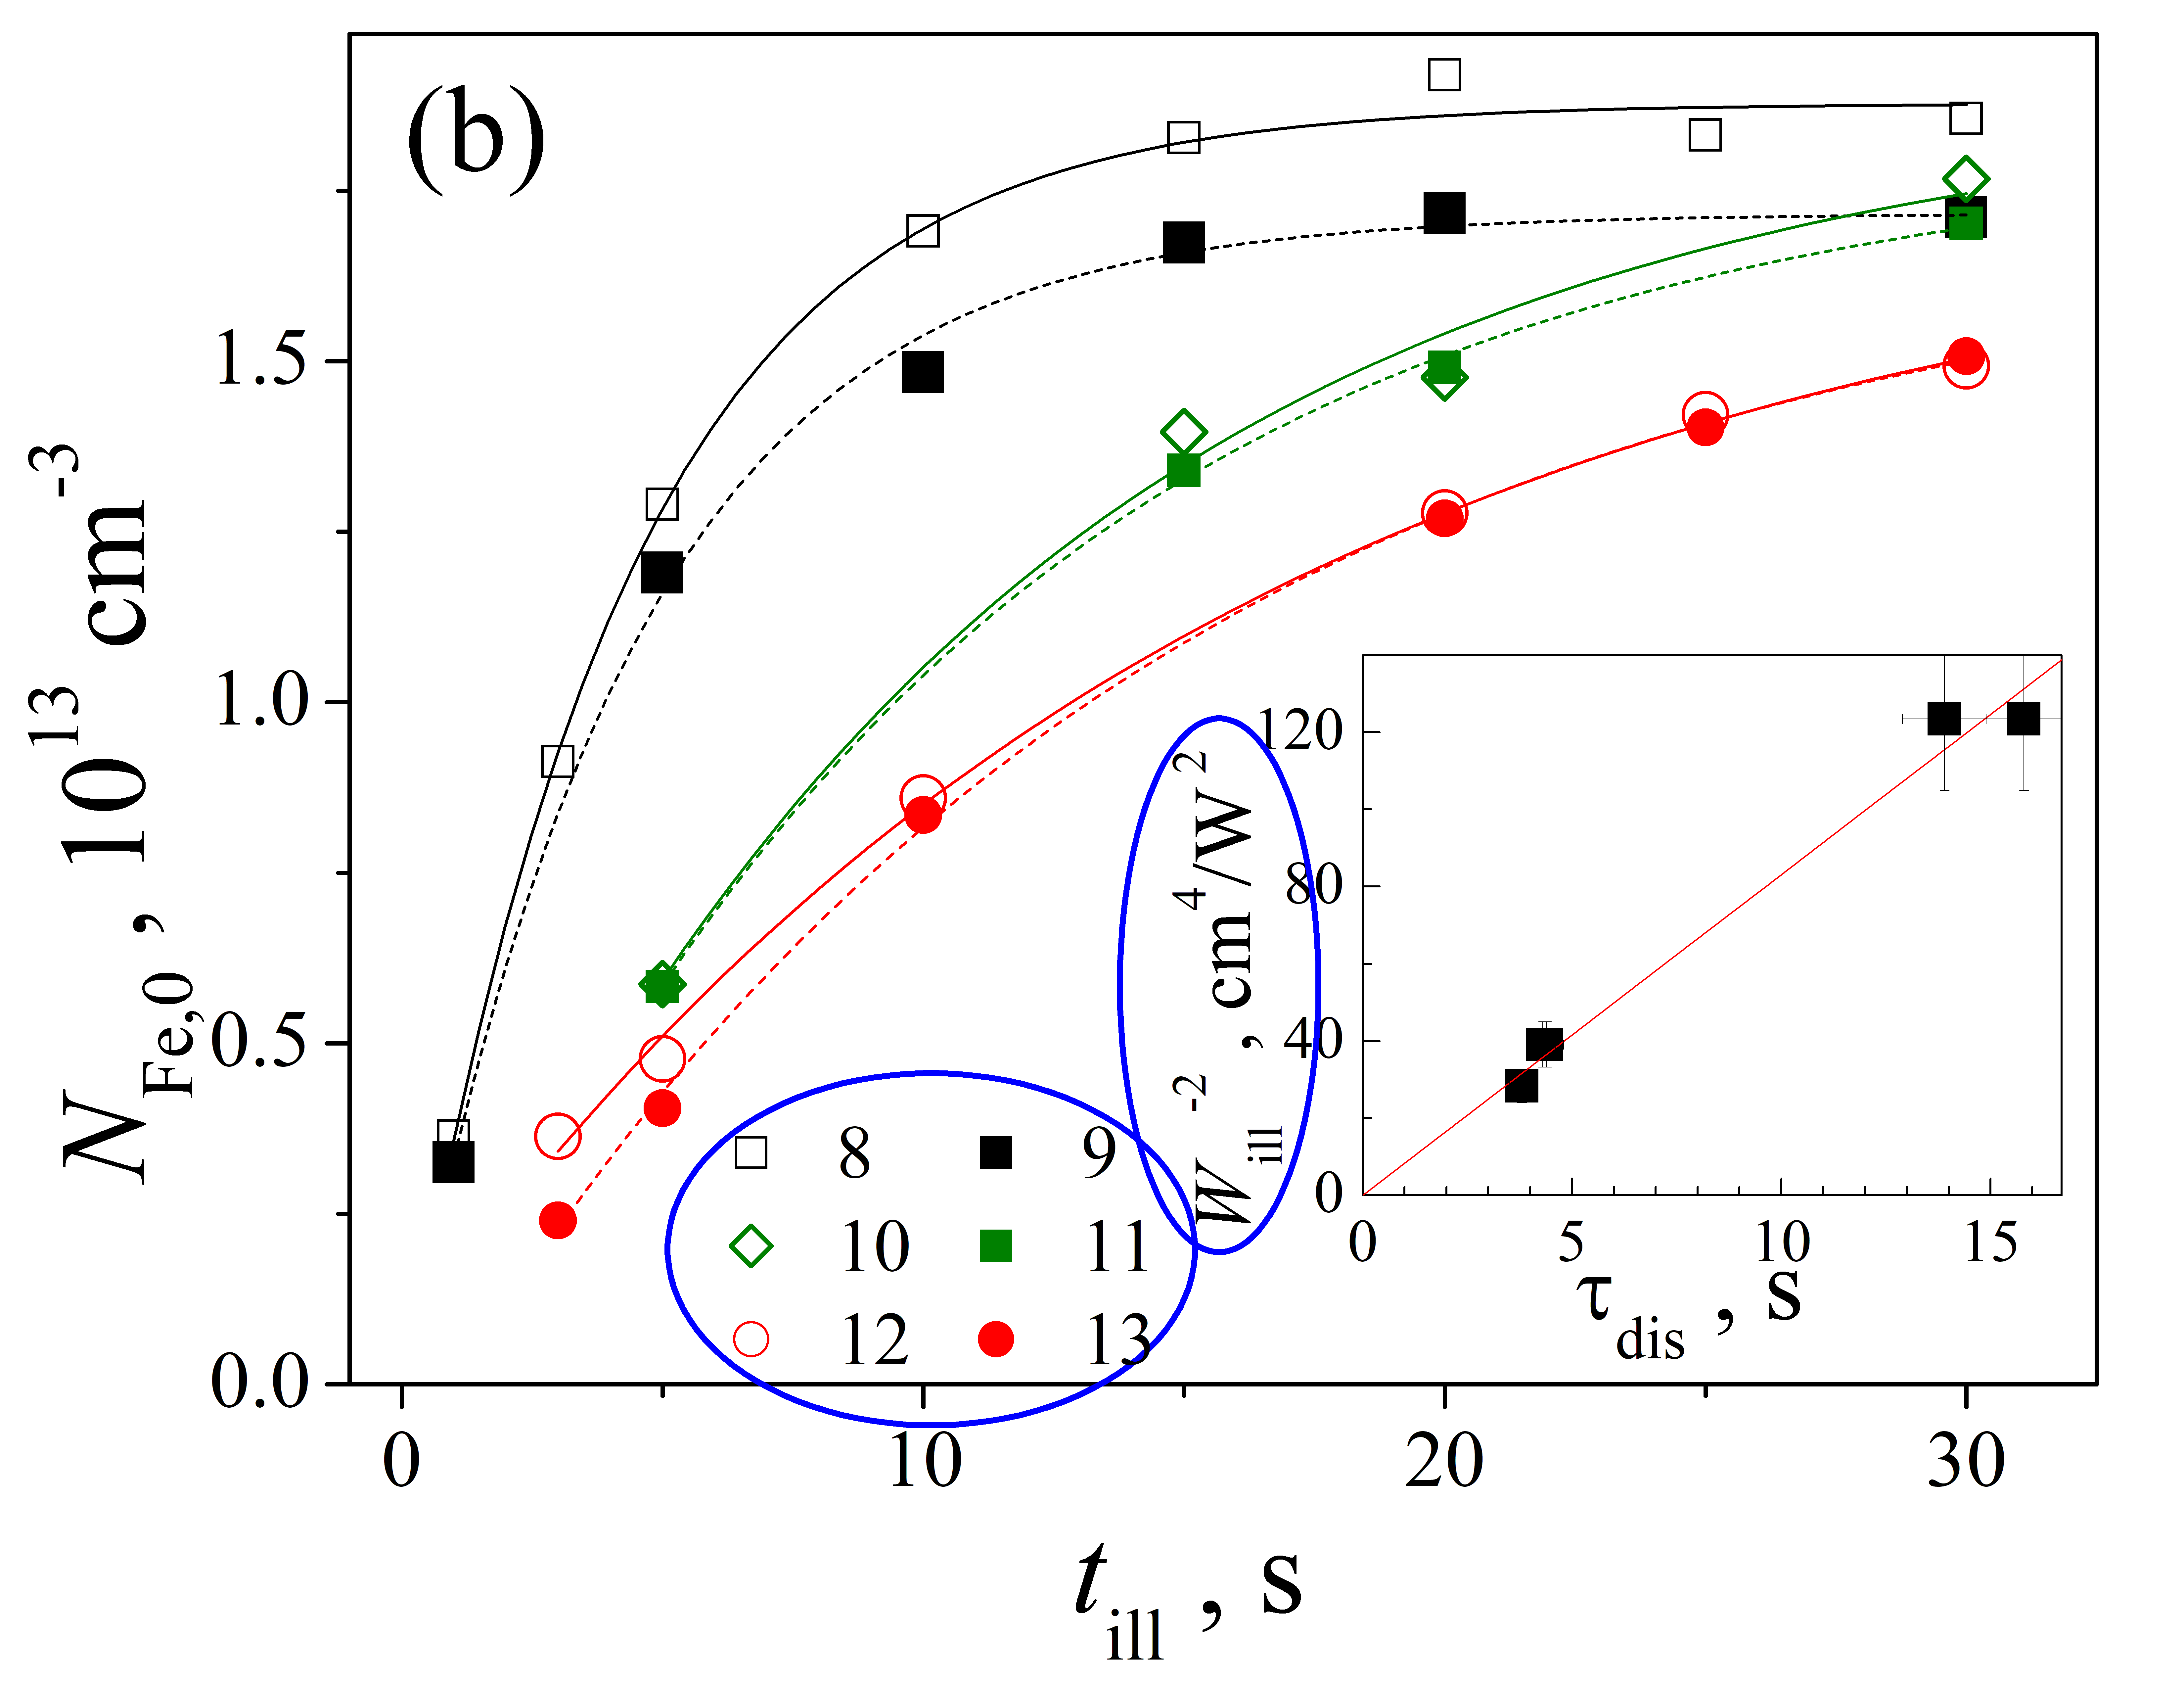
\includegraphics[width=0.33\textwidth]{Fig4b}% Here is how to import EPS art

\includegraphics[width=0.33\textwidth]{Fig4c}% Here is how to import EPS art
\caption{\label{Fig:Nfe_till}
Concentration dependence of interstitial atoms due to light induced dissociation on illumination time.
The marks are the experimental results, the lines are the curves  fitted by using Eq.~(\ref{eqNfe0Exp}).
Empty circles and solid lines are used for  the case without USL,
filled circles and dashed lines --- for the case of USL.
$W_\mathrm{ill}$, W/cm$^2$: 0.16 (curves 1-3, 8-11, 14, 15),
0.12 (4, 5, 16, 17), 0,09 (12, 13), 0.08 (6,7,18,19).
$W_\mathrm{US}$, W/cm$^2$:
0.9 (2, 5, 7), 0.6 (3, 9, 11, 13), 0.1 (15, 17, 19).
$f_\mathrm{US}$, MHz:
9,0 (2, 3, 5, 7), 0.3 (9, 11, 13), 5,0 (15, 17, 19);
$T$, K:
340 (1-9,12-19), 320 (10,11).
Samples SC350-1 (a), SC350-2 (b), SC349-1 (c).
Insets: $\tau_\mathrm{dis}$ are plotted against $W_\mathrm{ill}^{-2}$.
The lines are the curves fitted by $\tau_\mathrm{dis}=const\cdot W_\mathrm{ill}^{-2}$.
}
\end{figure*}


The obtained results show that as the illumination time grows
the values of $N_\mathrm{Fe,0}$ increase gradually until reaching saturation.
This is in complete correspondence with the results of the previous researches \cite{FeBLight2,FeBAssJAP2014,FeBKin2019}
that predict \textcolor[rgb]{0.00,0.07,1.00}{\uline{the}}
exponential decrease of pair concentration with the increase of illumination time.
The saturation should correspond to the condition of complete pair dissociation.
The experimentally obtained dependencies were approximated by using the following equation
\begin{equation}
\label{eqNfe0Exp}
N_\mathrm{Fe,0}(t_\mathrm{ill})=A\exp(-t_\mathrm{ill}/\tau_\mathrm{dis})
+N_\mathrm{Fe,fit}\,,
\end{equation}
where
$\tau_\mathrm{dis}$ is the characteristic time of dissociation,
$N_\mathrm{Fe,fit}$ is the value corresponding to saturation.
The examples of approximation curves are given in Fig.~\ref{Fig:Nfe_till},
and the values of the parameters obtained by approximation --- in
\textcolor[rgb]{0.00,0.07,1.00}{\uline{
Table~\ref{tabSample}.}}
%Fig.~\ref{Fig:IllRez}.

\textcolor[rgb]{0.00,0.07,1.00}{
\begin{table}
\caption{\label{tabSample}The value of maximum concentrations of light released iron atoms
and characteristic dissociation time obtained by approximating experimental dependencies by Eq.~(\ref{eqNfe0Exp}).
}
\begin{ruledtabular}
\begin{tabular}{ccccccc}
\multirow{2}{*}{Sample} &$T$&$W_\mathrm{ill}$&$f_\mathrm{US}$&$W_\mathrm{US}$& $N_\mathrm{Fe,fit}$
&$\tau_\mathrm{dis}$ \\
&(K)& (W/cm$^2$)& (MHz)&(W/cm$^2$)&($10^{13}$~cm$^{-3})$&(s) \\
\hline
SC350-1&340&0.08&\multicolumn{2}{c}{non}&$3.0\pm0.3$&$15\pm4$\\
&340&0.08&9.0&0.9&$2.9\pm0.4$&$15\pm6$\\
&340&0.12&\multicolumn{2}{c}{non}&$2.98\pm0.07$&$7\pm1$\\
&340&0.12&9.0&0.9&$2.99\pm0.06$&$7\pm1$\\
&340&0.16&\multicolumn{2}{c}{non}&$2.98\pm0.02$&$3.4\pm0.2$\\
&340&0.16&9.0&0.6&$2.78\pm0.03$&$3.1\pm0.6$\\
&340&0.16&9.0&0.9&$2.67\pm0.07$&$2.9\pm0.6$\\
SC352-1&340&0.16&\multicolumn{2}{c}{non}&$4.25\pm0.03$&$3.8\pm0.2$\\
&340&0.16&5.9&1.0&$4.03\pm0.04$&$3.7\pm0.2$\\
SC350-2&340&0.09&\multicolumn{2}{c}{non}&$1.76\pm0.08$&$16\pm2$\\
&340&0.09&0.3&0.6&$1.72\pm0.05$&$14\pm1$\\
&340&0.12&\multicolumn{2}{c}{non}&$1.89\pm0.02$&$9\pm1$\\
&340&0.12&0.3&0.6&$1.86\pm0.03$&$8\pm2$\\
&340&0.16&\multicolumn{2}{c}{non}&$1.88\pm0.02$&$4.3\pm0.3$\\
&340&0.16&0.3&0.6&$1.72\pm0.02$&$4.4\pm0.4$\\
&320&0.16&\multicolumn{2}{c}{non}&$1.9\pm0.2$&$11\pm4$\\
&320&0.16&0.3&0.6&$1.8\pm0.1$&$11\pm1$\\
SC349-1&340&0.08&\multicolumn{2}{c}{non}&$0.66\pm0.02$&$7\pm1$\\
&340&0.08&5.0&0.5&$0.64\pm0.05$&$9\pm3$\\
&340&0.12&\multicolumn{2}{c}{non}&$0.65\pm0.01$&$2.7\pm0.3$\\
&340&0.12&5.0&0.5&$0.62\pm0.01$&$2.9\pm0.4$\\
&340&0.16&\multicolumn{2}{c}{non}&$0.67\pm0.01$&$2.3\pm0.2$\\
&340&0.16&5.0&0.5&$0.61\pm0.01$&$1.8\pm0.3$\\
\end{tabular}
\end{ruledtabular}
\end{table}
}

%\begin{figure}
%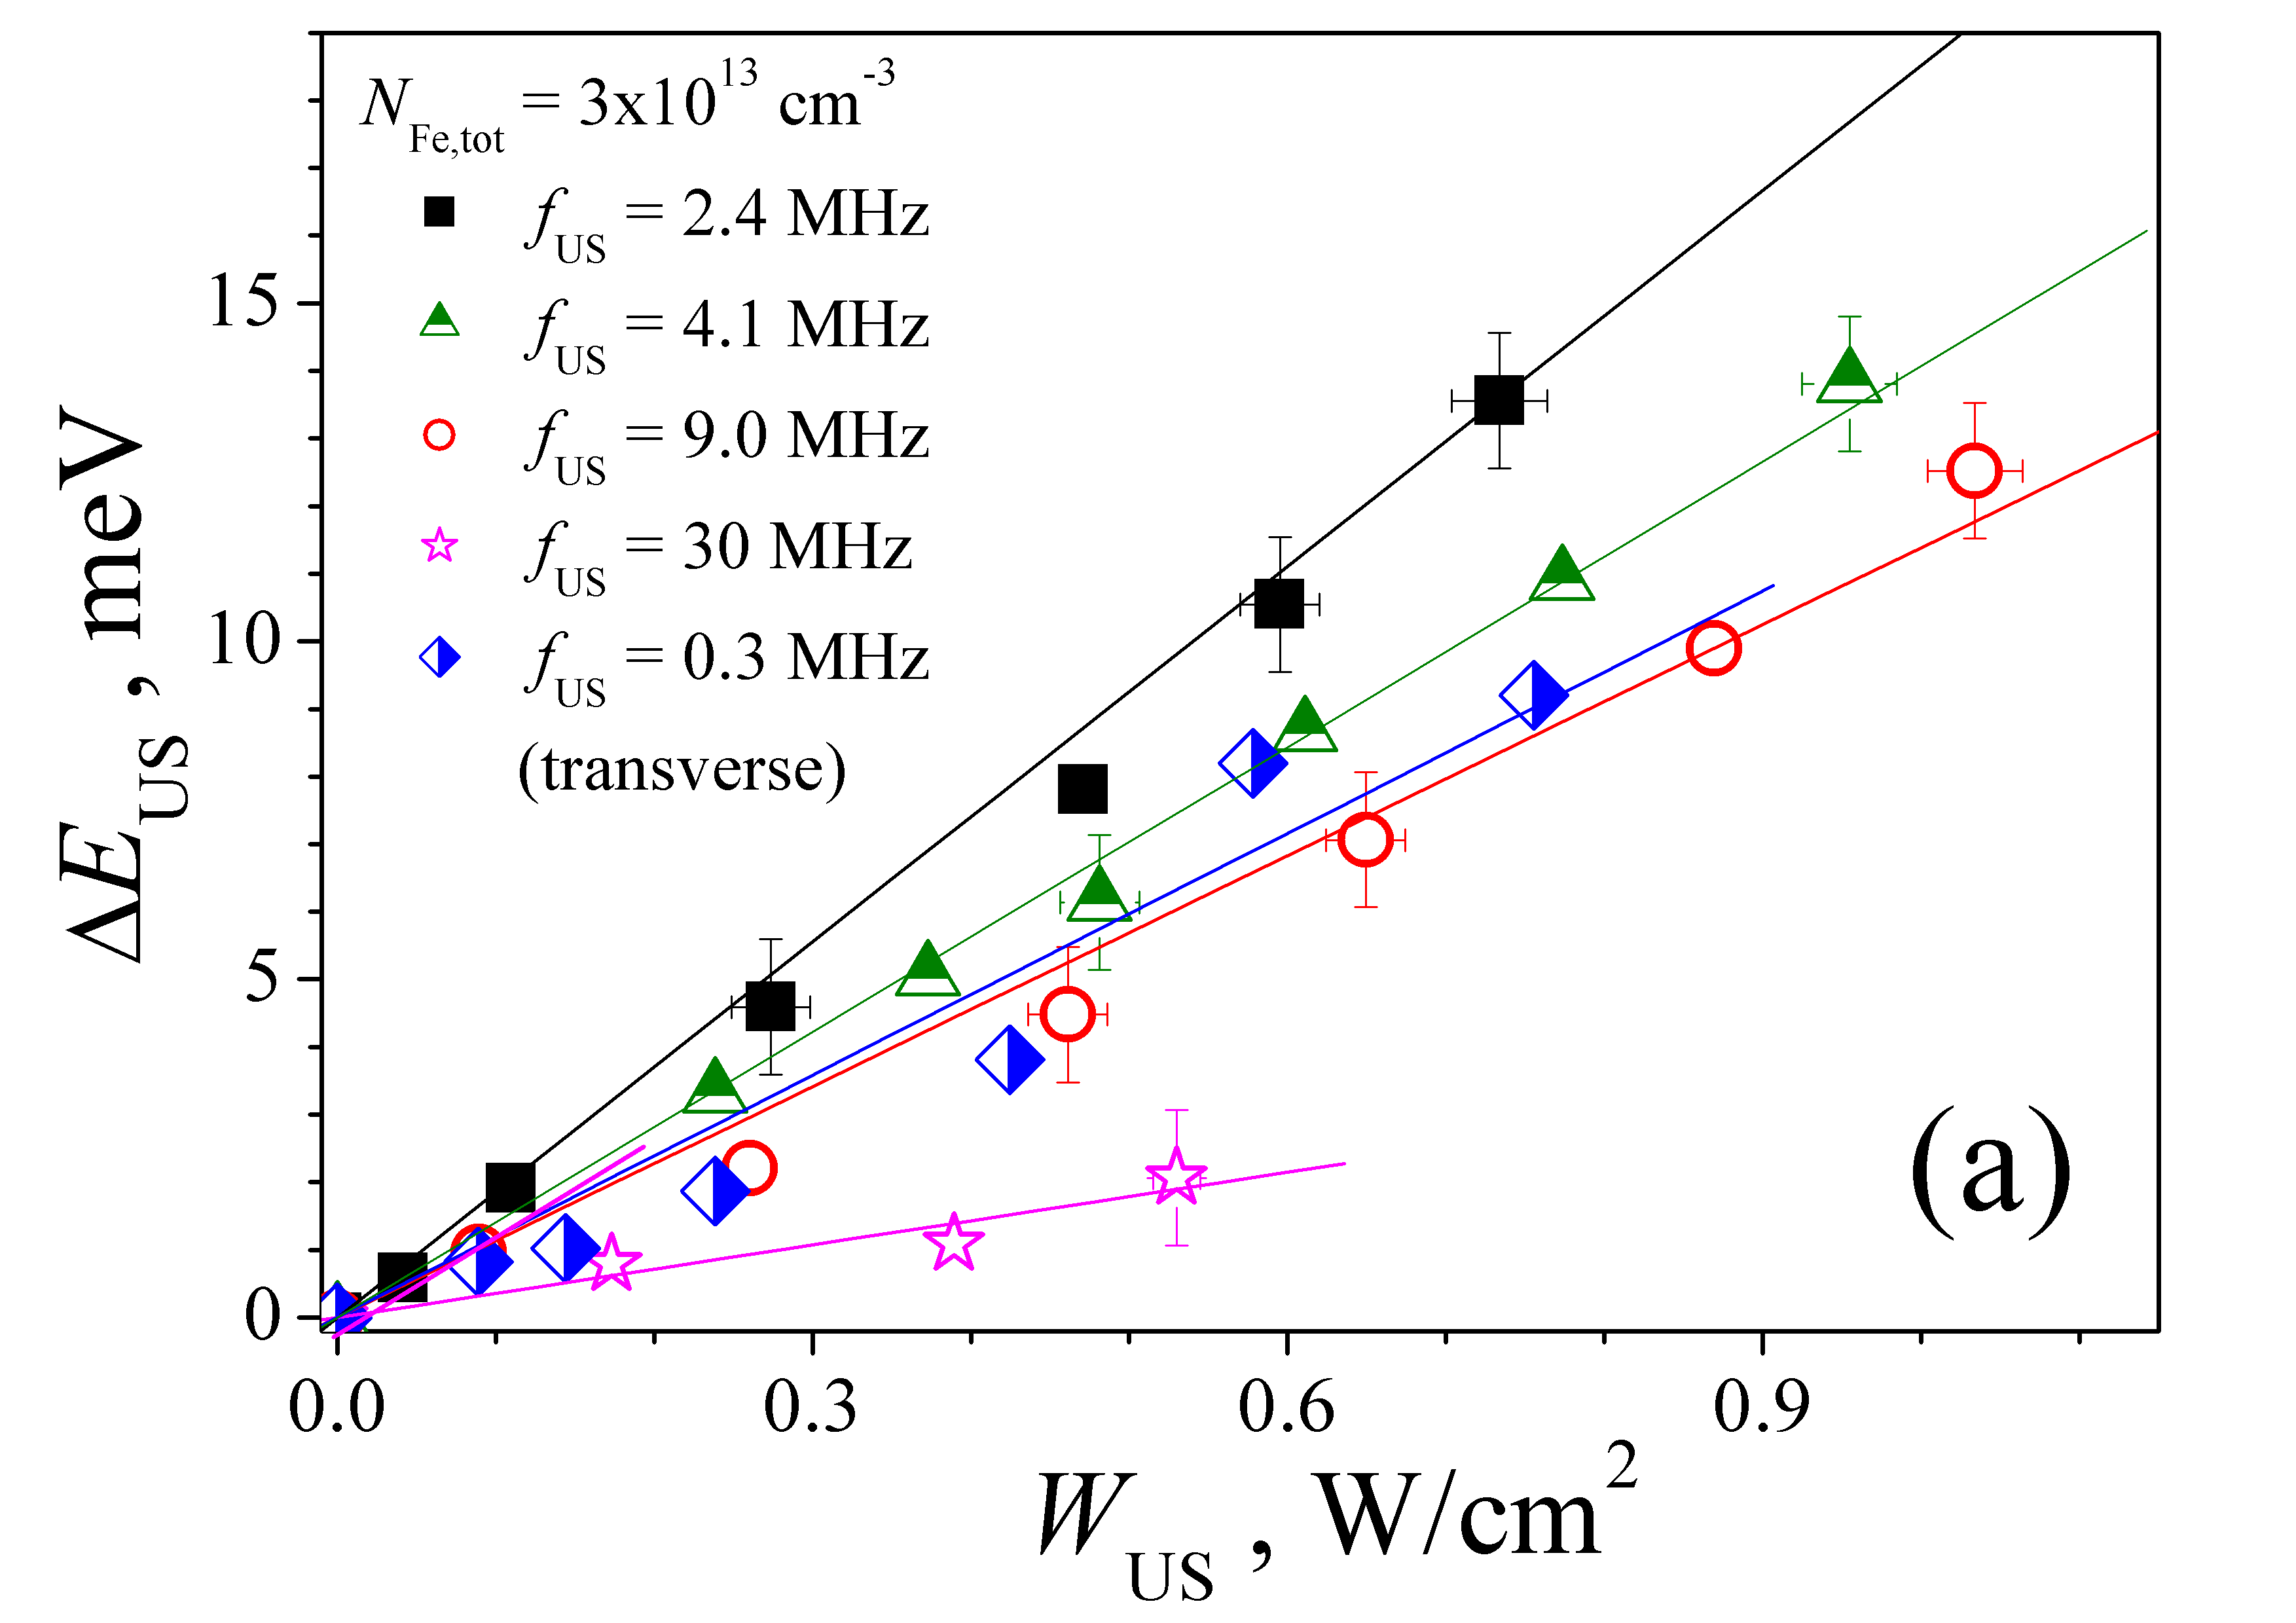
\includegraphics[width=0.5\textwidth]{Fig5a}\\% Here is how to import EPS art
%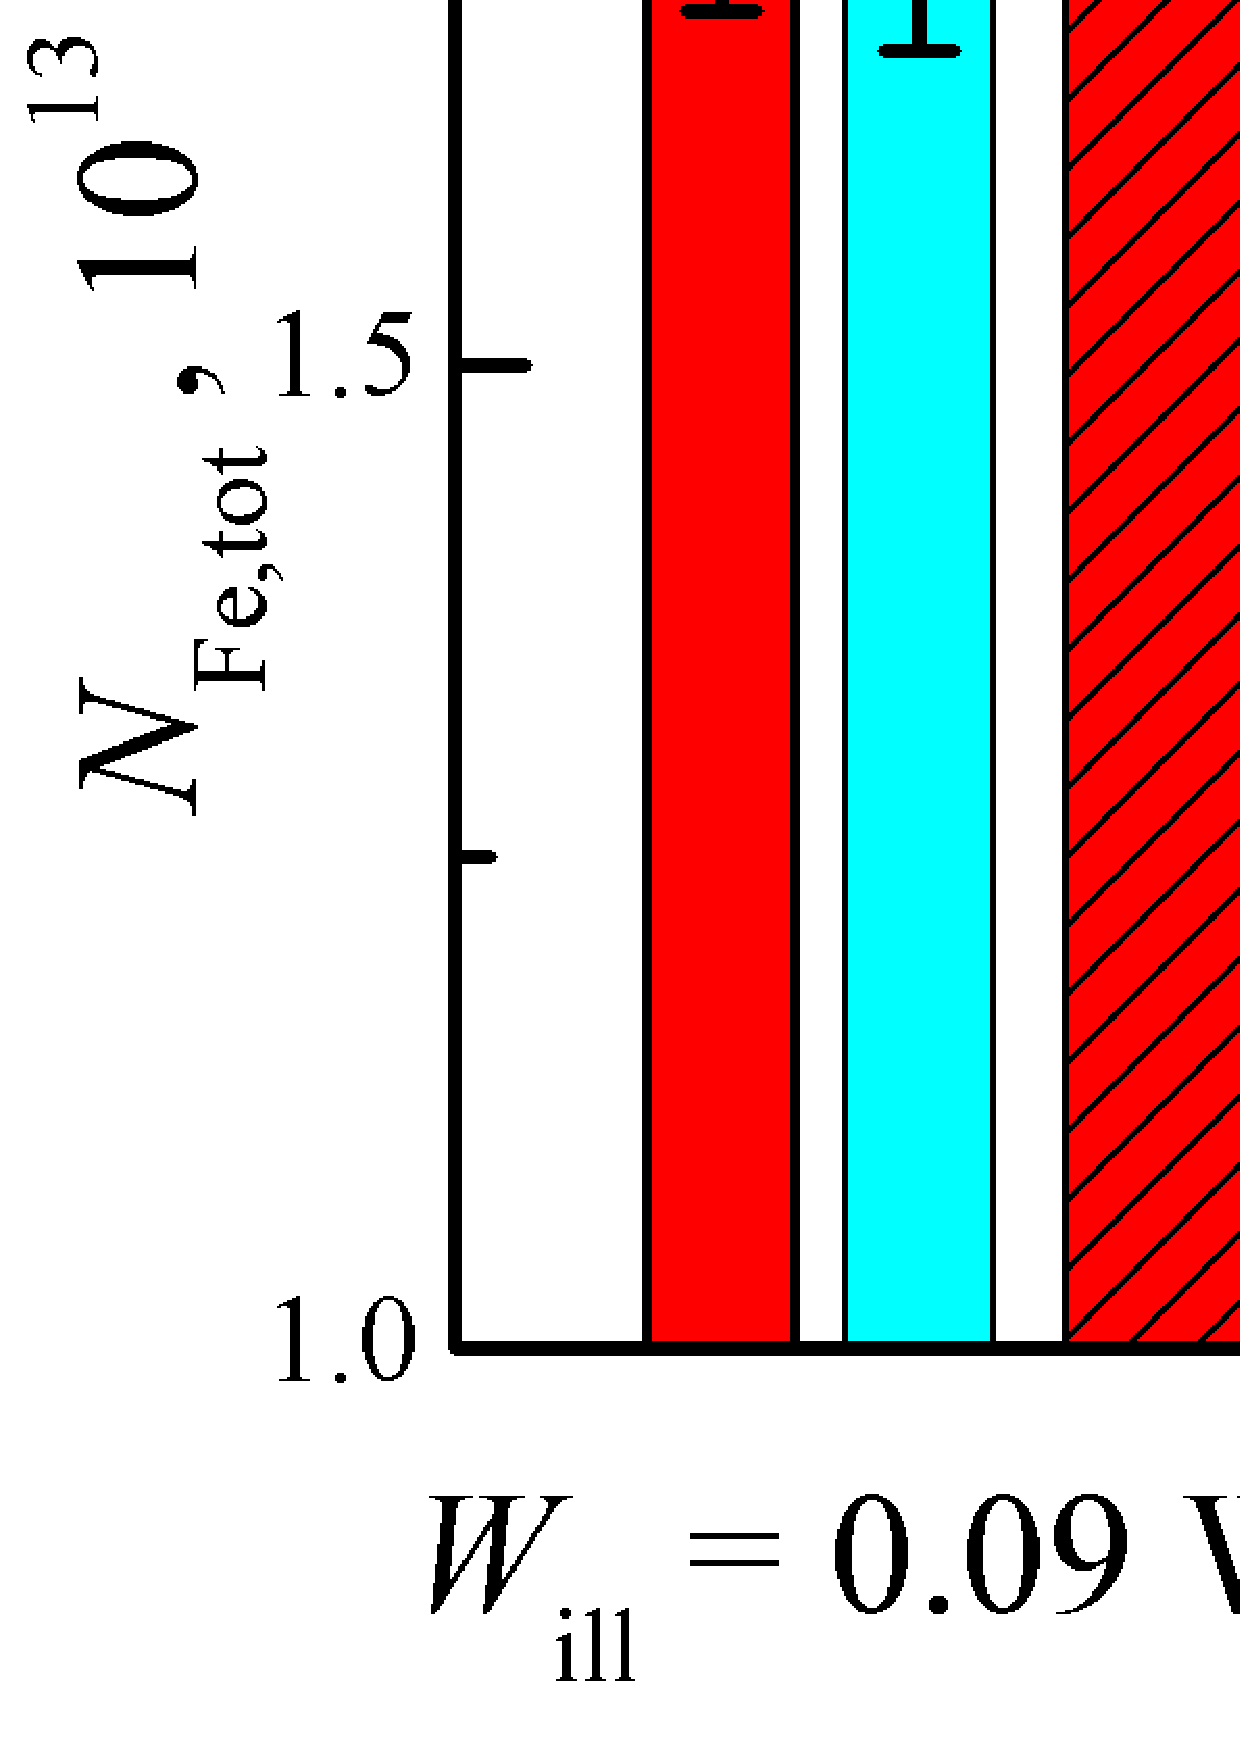
\includegraphics[width=0.5\textwidth]{Fig5b}\\% Here is how to import EPS art
%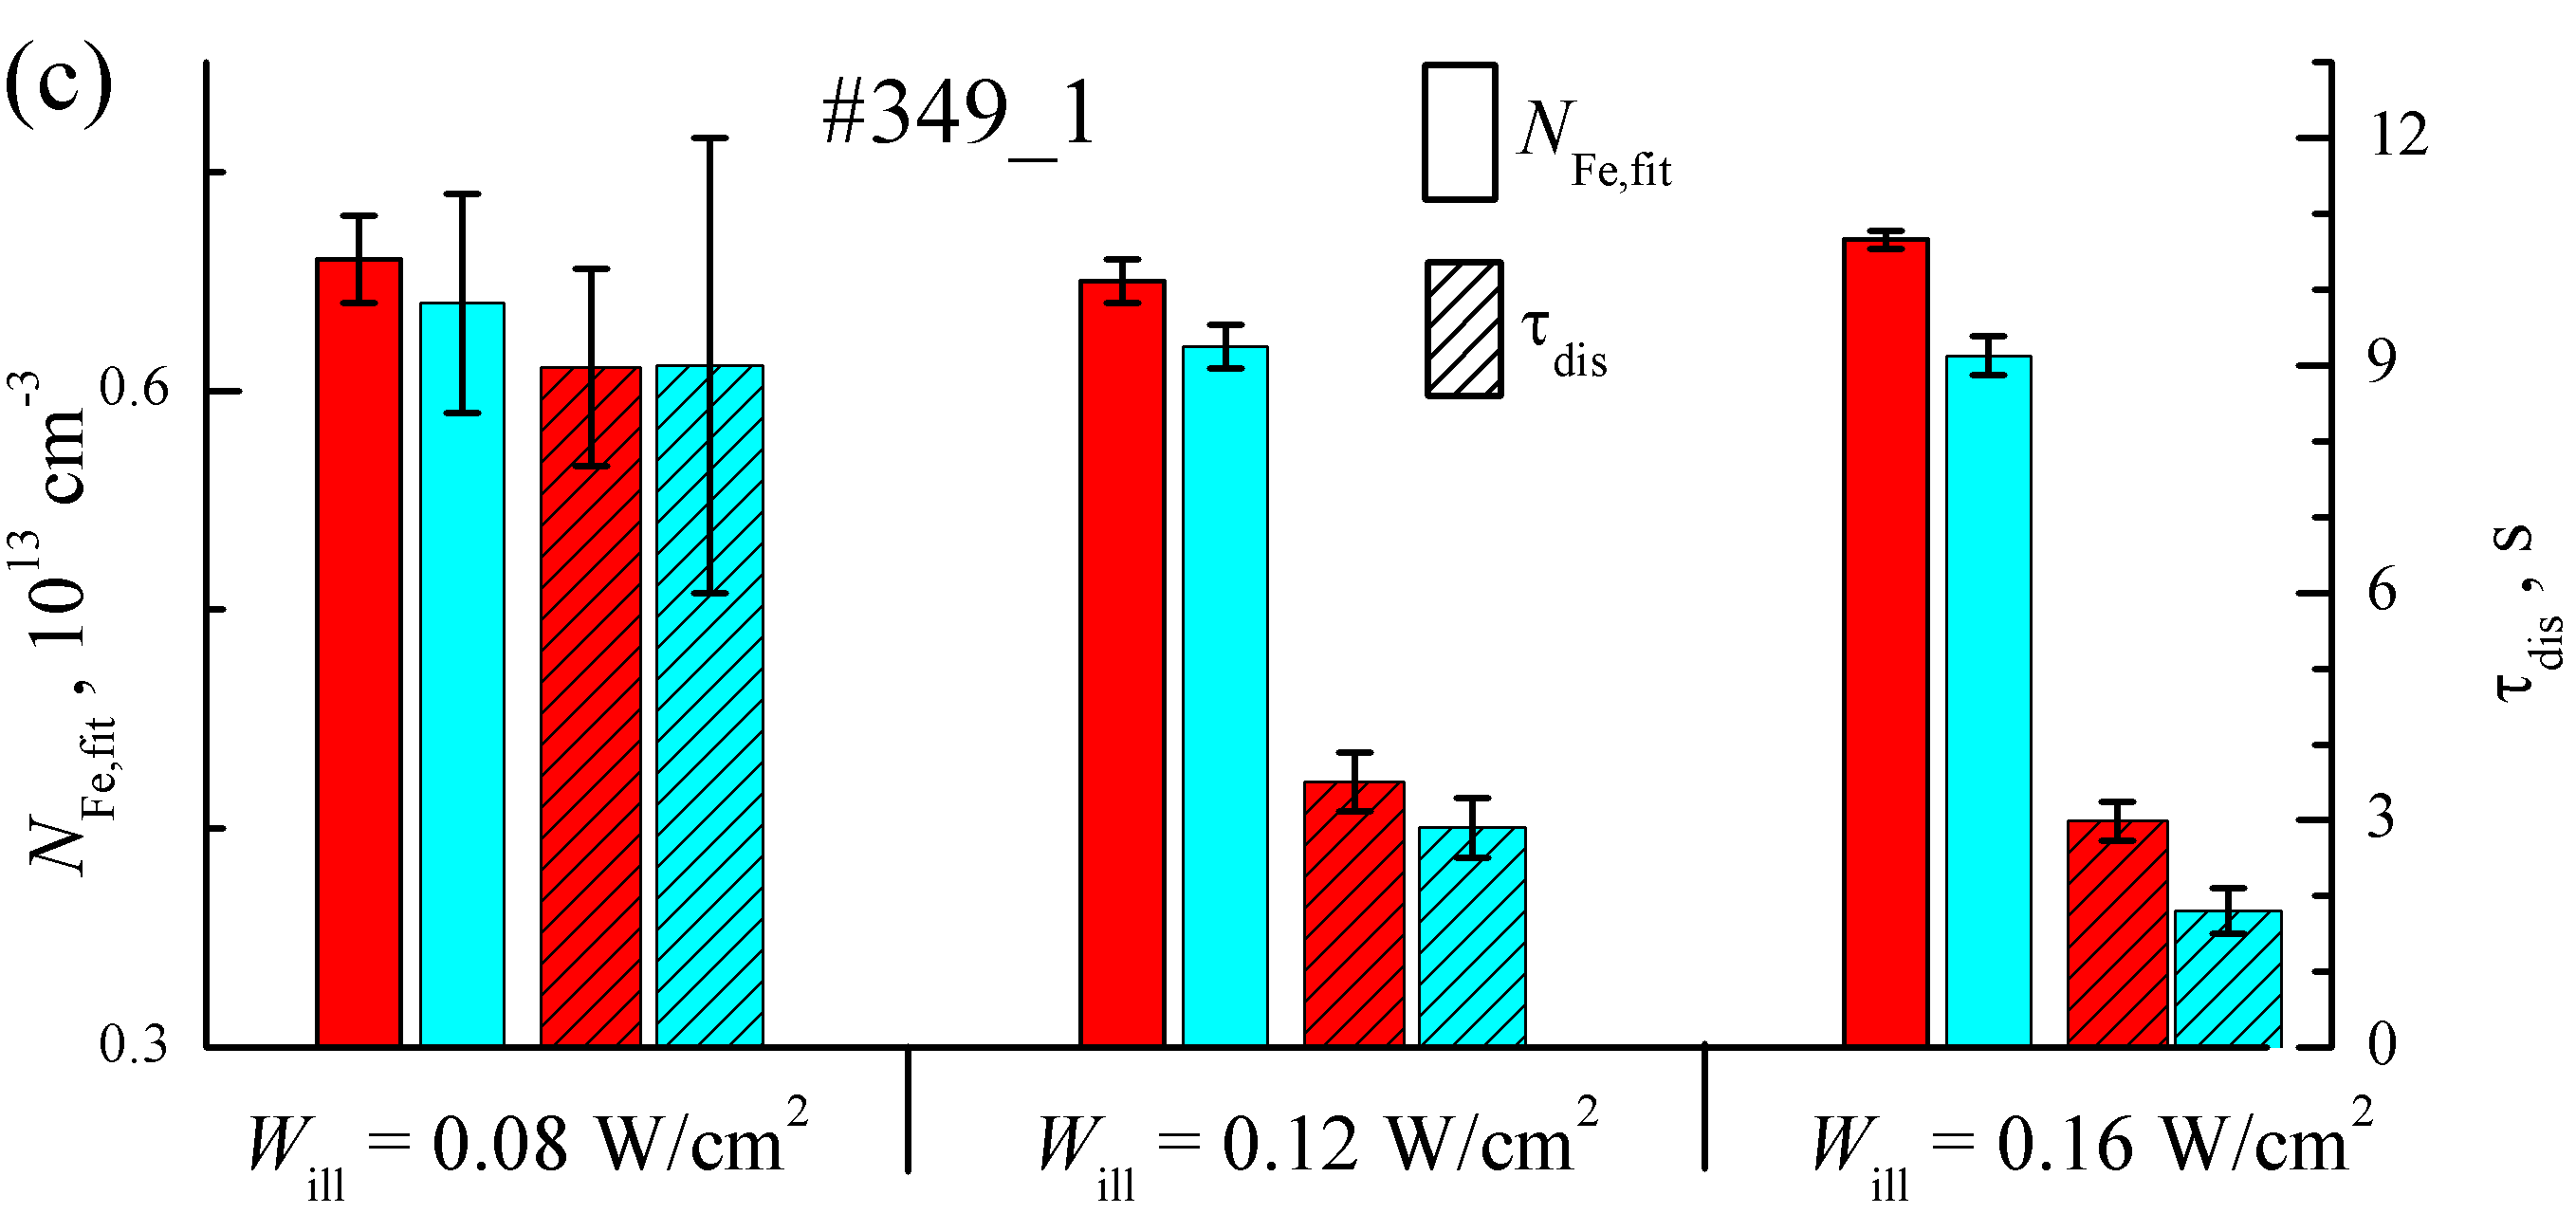
\includegraphics[width=0.5\textwidth]{Fig5c}% Here is how to import EPS art
%\caption{\label{Fig:IllRez}
%The value of maximum concentrations of light released iron atoms (unhatched bars)
%and characteristic dissociation time (hatched bars) obtained by approximating experimental dependencies by Eq.~(\ref{eqNfe0Exp}).
%Red bars correspond to cases without USL,
%blue ones --- with USL.
%Violet and pink bars (panel b) are obtained at $T=320$~K,
%the rest --- at $T=340$~K.
%The conditions of USL for samples SC350-1, SC350-2,
%SC349-1 are identical with those given in the caption to Fig.~\ref{Fig:Nfe_till}.
%For SC352-1 $f_\mathrm{US}=5.9$~MHz,
%$W_\mathrm{US}=1.0$~W/cm$^2$.
%}
%\end{figure}

On the other way,
the equilibrium between free Fe$_i$ and Fe$_i$B$_s$ is determined by the following rate equations
\begin{eqnarray}
\label{eqkinet}
\mathrm{Fe}_i+\mathrm{B}_s\xrightarrow{R_a}\mathrm{FeB}\,,\nonumber\\
\mathrm{FeB}\xrightarrow{R_d}\mathrm{Fe}_i+\mathrm{B}_s\,,
\end{eqnarray}
where
$R_a=\tau_\mathrm{ass}^{-1}$ and
$R_d$ are the association and dissociation rates of FeB pairs, respectively.
From Eq.~(\ref{eqkinet}), taking into account that
$N_\mathrm{Fe}=N_\mathrm{Fe,tot}-N_\mathrm{FeB}$
and
$N_\mathrm{Fe}(t_\mathrm{ill}=0)=N_\mathrm{Fe,eq}$,
the time dependent interstitial iron content during illumination can be described as follows
%\begin{equation}
%\label{eqNfeill}
%N_\mathrm{Fe}(t_\mathrm{ill})=\left(N_\mathrm{Fe,eq}-N_\mathrm{Fe,tot}
%\frac{R_d}{R_d+R_a}\right)\exp[-(R_d+R_a)t_\mathrm{ill}]
%+N_\mathrm{Fe,tot}\frac{R_d}{R_d+R_a}\,.
%\end{equation}
\begin{eqnarray}
\label{eqNfeill}
N_\mathrm{Fe}(t_\mathrm{ill})&=&\left(N_\mathrm{Fe,eq}-N_\mathrm{Fe,tot}
\frac{R_d}{R_d+R_a}\right)\exp[-(R_d+R_a)t_\mathrm{ill}]+\nonumber\\
&&N_\mathrm{Fe,tot}\frac{R_d}{R_d+R_a}\,.
\end{eqnarray}
The comparison of Eqs.~(\ref{eqNfe0Exp}) and (\ref{eqNfeill}) shows that
$\tau_\mathrm{dis}^{-1}=R_a+R_d$,
$N_\mathrm{Fe,fit}=N_\mathrm{Fe,tot}R_d/(R_a+R_dKd)$.
It should be noted that in our case
(see Sec.~\ref{sec:FeBass}) $\tau_\mathrm{ass}\gg \tau_\mathrm{dis}$
(without USL $\tau_\mathrm{ass}\simeq700$~s at 340~K and $\tau_\mathrm{ass}\simeq13000$~s at 300~K). Therefore, $R_d\gg>>R_a$ and $\tau_\mathrm{dis}^{-1}\simeq R_d$,
$N_\mathrm{Fe,fit}\simeq N_\mathrm{Fe,tot}$.

As for the case without USL, we should note the following.
First, for every sample $N_\mathrm{Fe,fit}$ remains constant and does not depend on illumination intensity and temperature
\textcolor[rgb]{0.00,0.07,1.00}{\uline{
--- see Table~\ref{tabSample}.}}
%(red and pink unhatched bars in Fig.~\ref{Fig:IllRez}).
This is quite expectable if we assume that
in this case $N_\mathrm{Fe,fit}=N_\mathrm{Fe,tot}$.
Second, the value of $\tau_\mathrm{dis}$
\textcolor[rgb]{0.00,0.07,1.00}{\uline{
(last column in Table~\ref{tabSample})
}}
%(hatched bars in Fig.~\ref{Fig:IllRez})
depends on $W_\mathrm{ill}$ and $T$.
It is well known \cite{Schmidt2019,FeBLight2,FeBKin2019} that the dissociation rate of FeB pairs increases quadratically with increasing illumination intensity.
In the insets in Fig.~\ref{Fig:Nfe_till} the values of $\tau_\mathrm{dis}$
are plotted against $W_\mathrm{ill}^{-2}$.
The linearity of the obtained curves is in a complete coincidence
with the reported data and can serve as \textcolor[rgb]{0.00,0.07,1.00}{\uline{an}} additional proof of the suggested approach
applicability in estimating iron-related defect parameters.
Moreover, it is known \cite{Lagowskii1993} that the dissociation time decreases approximately twice per 20$^\circ$C increase.
In our experiment, $\tau_\mathrm{dis}=(11\pm4)$~s for sample SC350-2
(Figs.~\ref{Fig:Nfe_till}(b) and
\textcolor[rgb]{0.00,0.07,1.00}{\uline{
Table~\ref{tabSample}}}
%~\ref{Fig:IllRez}(b)
) at $T=320$~K , and at 340~K,
it comprised $4.3\pm0.3$~s, which justifies the expectations.

Another reason why it is advisable to analyze $I\mathrm{SC}$ kinetics is the behavior of
$\tau_\mathrm{other}$ revealed in the experiments.
In the case when $\tau_\mathrm{ill}$ corresponds to the values of $N_\mathrm{Fe,0}$ close to saturation, the other recombination channels  can be neglected ($\tau_\mathrm{other}> 100$~ms).
In the case when the values of $t_\mathrm{ill}$ are small,
$\tau_\mathrm{other}$ changes in the range $10^{-6}-10^{-4}$~s \textcolor[rgb]{0.00,0.07,1.00}{\uline{and begins}} to increase as the illumination time increases.
In terms of the proposed approximation, this indicates that some parts of FeB pairs have not dissociated and the value of $\tau_\mathrm{other}$ is related
to recombination on iron-related defects that do not reconstruct when the sample is kept in darkness. In order to support this assumption the quantity
$\tau_\mathrm{other}^\mathrm{calc}$
was estimated as follows
\begin{equation*}
\tau_\mathrm{other}^\mathrm{calc}=\left(\left(\tau_{SRH}^\mathrm{Fe_i}\right)^{-1}
+\left(\tau_{SRH}^\mathrm{FeB}\right)^{-1}\right)^{-1}
\end{equation*}
where
$\tau_{SRH}^\mathrm{Fe_i}$ and $\tau_{SRH}^\mathrm{FeB}$
were calculated by Eq.~(\ref{eqTauSRH}) for defect concentrations
$N_\mathrm{Fe}=N_\mathrm{Fe,eq}(N_\mathrm{Fe,tot}-N_\mathrm{Fe,0})$
and $N_\mathrm{FeB}= N_\mathrm{Fe,tot}-N_\mathrm{Fe,0}- N_\mathrm{Fe}$, accordingly.
 \textcolor[rgb]{0.00,0.07,1.00}{\uline{
It turned out that $\tau_\mathrm{other}^\mathrm{calc}$ and
$\tau_\mathrm{other}$, obtained in the same conditions, are very close:
the correlation coefficient equals to 0.98 (see Supplementary Material).
}}

Paying our attention back to the impact of acoustic waves on the processes of light--induced dissociation of FeB pairs, the following should be noted.
First,  USL actually does not influence the magnitude of
\textcolor[rgb]{0.00,0.07,1.00}{\uline{
dissociation time:
$\tau_\mathrm{dis}$ values in neighboring rows}}
%the heights of neighboring hatched red and blue bars
are similar in the error range for all the cases in
\textcolor[rgb]{0.00,0.07,1.00}{\uline{
Table~\ref{tabSample}}}.
%Fig.~\ref{Fig:IllRez} .
Second, some pairs do not dissociate under \textcolor[rgb]{0.00,0.07,1.00}{\uline{illumination in the USL case}}:
$N_\mathrm{Fe,fit}(W_\mathrm{US}>0)< N_\mathrm{Fe,fit}(W_\mathrm{US}=0)$.
How large the portion of these pairs is, depends on US intensity
(see Figs.~\ref{Fig:Nfe_till}(a),
\textcolor[rgb]{0.00,0.07,1.00}{\uline{
Table~\ref{tabSample}}},
%\ref{Fig:IllRez}(a),
$W_\mathrm{ill}=0.16$~W/cm$^2$);
and at maximum $W_\mathrm{US}$ values this portion reaches 10\%.
It should be noted that this [effect] is observed only in the case when light--induced pair dissociation is close to saturation.
If $W_\mathrm{ill}$ (or temperature), however, is that \textcolor[rgb]{0.00,0.07,1.00}{\uline{at which}}
a part of iron atoms stays near the substitutional boron atoms at the given illumination times,
then $N_\mathrm{Fe,fit}(W_\mathrm{US}>0)\simeq N_\mathrm{Fe,fit}(W_\mathrm{US}=0)$.


\subsection{\label{sec:FeBass}FeB association}

It has also been found that USL accelerates FeB pair association --–
see. Fig.~\ref{Fig:IscKin}(b).
As seen from the figure, the main result of ultrasound excitation in the structure
is the decrease in time of short circuit current recovery.
Since in approximating experimental dependencies $I_\mathrm{SC}(t)$ we assumed that pre--exponential multiplier in Eq.~(\ref{eqTass}) does not depend on USL
(but relies only on the temperature and level of base doping),
\textcolor[rgb]{0.00,0.07,1.00}{\uline{in order}} to find numerical characteristics of this effect,
we used the change in migration energy $\Delta E_\mathrm{US}$, i.e., it was assumed that
\begin{equation}
\label{eqEmUs}
E_m \xrightarrow{ultrasound} E_{m,0}-\Delta E_\mathrm{US}\,,
\end{equation}
where $E_{m,0}$ is the migration energy estimated without USL,
$\Delta E_\mathrm{US}$ is the acoustically induced (AI) change in migration energy.
It is seen from Fig.~\ref{Fig:IscKin}(b)
that $\Delta E_\mathrm{US}$ depends on acoustic wave intensity.
Fig.~\ref{Fig:EmWus} presents the dependencies $\Delta E_\mathrm{US}=\Delta E_\mathrm{US}(W_\mathrm{US})$ at varied US frequencies and for the samples with different iron content
(estimated by the dependencies similar to those given in Fig.~\ref{Fig:Nfe_till}).
The presented data show that

\begin{figure}
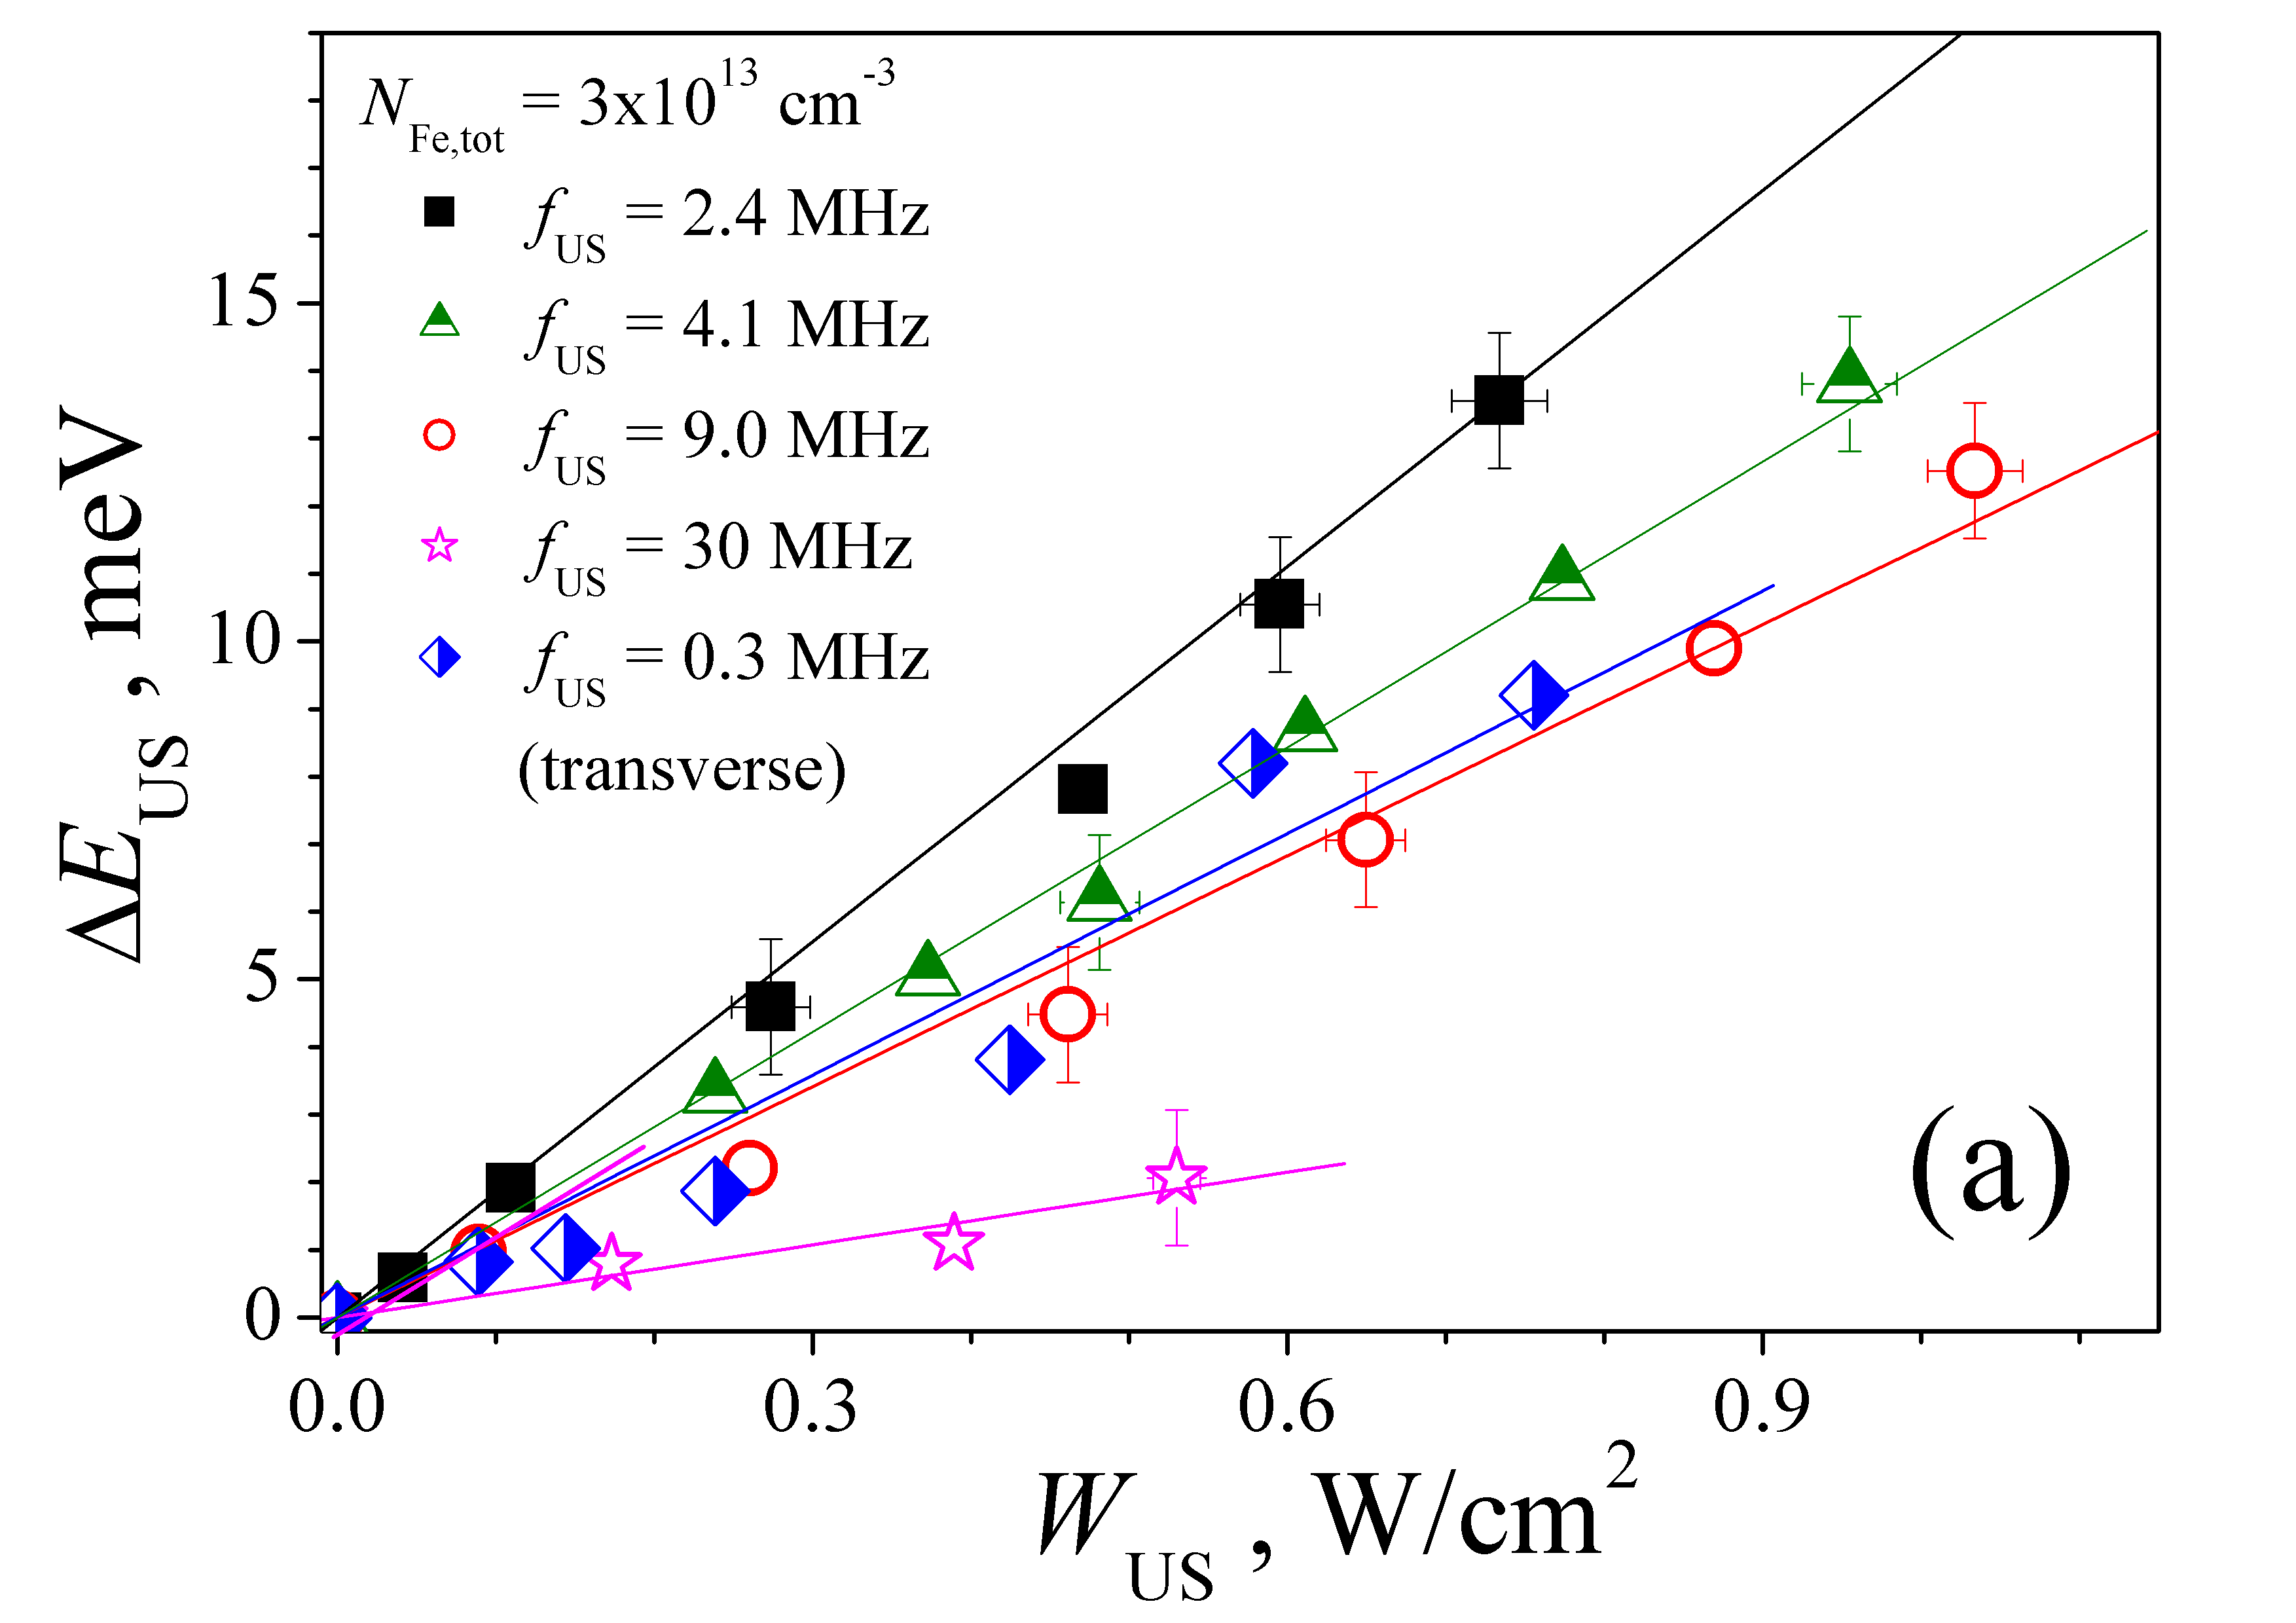
\includegraphics[width=0.45\textwidth]{Fig5a}\\% Here is how to import EPS art
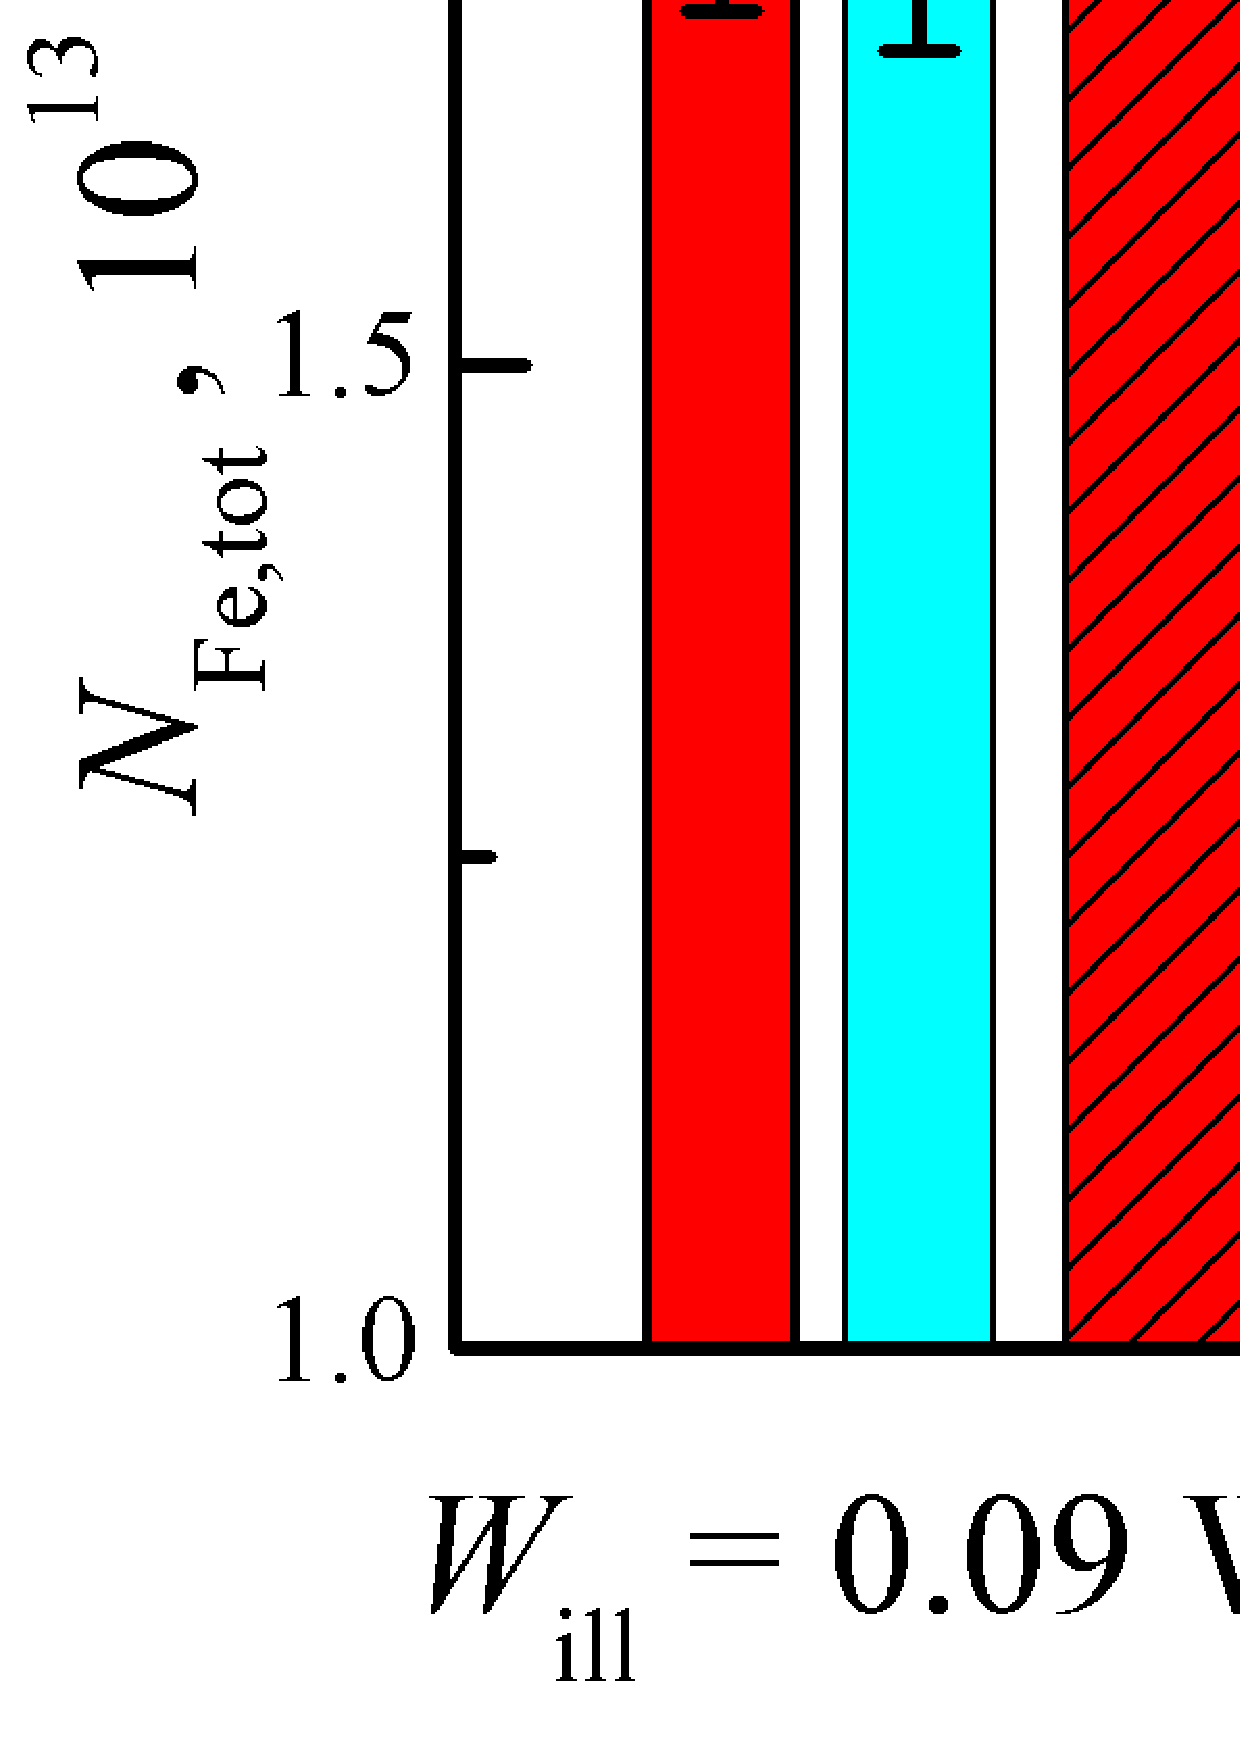
\includegraphics[width=0.45\textwidth]{Fig5b}% Here is how to import EPS art
\caption{\label{Fig:EmWus}
Dependencies of AI change in migration energy on US intensity for various
frequencies (a) and samples with different  iron concentrations (b).
$T=340$~K.
The points were obtained by approximating experimental dependencies,
the lines are the linear fitted curves.
}
\end{figure}


\begin{enumerate}
  \item $\Delta E_\mathrm{US}$ shows a practically linear dependence on US intensity;
  \item Effectiveness of AI change in migration energy decreases as the US frequency increases; transverse waves, despite their low frequency, less strongly impact the processes of iron ion diffusion;
  \item the magnitude of AI effect practically does not depend on iron concentration;
  \item AI change in migration energy can be as high as 13~meV.
\end{enumerate}

$\Delta E_\mathrm{US}$ has not been found to depend on illumination intensity.

The data presented in Fig.~\ref{Fig:EmWus} were obtained at 340~K.
With the decrease of temperature, the AI effect  decreases –-- see Fig.~\ref{Fig:EmT}.
As seen from the figure, temperature dependencies of $\Delta E_\mathrm{US}$ are close to linear:
\begin{equation}
\label{eqEmT}
\Delta E_\mathrm{US}(T)=\Delta E_\mathrm{US}(0)+\alpha_\mathrm{US}T\,,
\end{equation}
where temperature coefficient $\alpha_\mathrm{US}$ depends on US frequency
(see inset in Fig.~\ref{Fig:EmT}), while $\Delta E_\mathrm{US}(0)$ depends also on the US intensity.

\begin{figure}
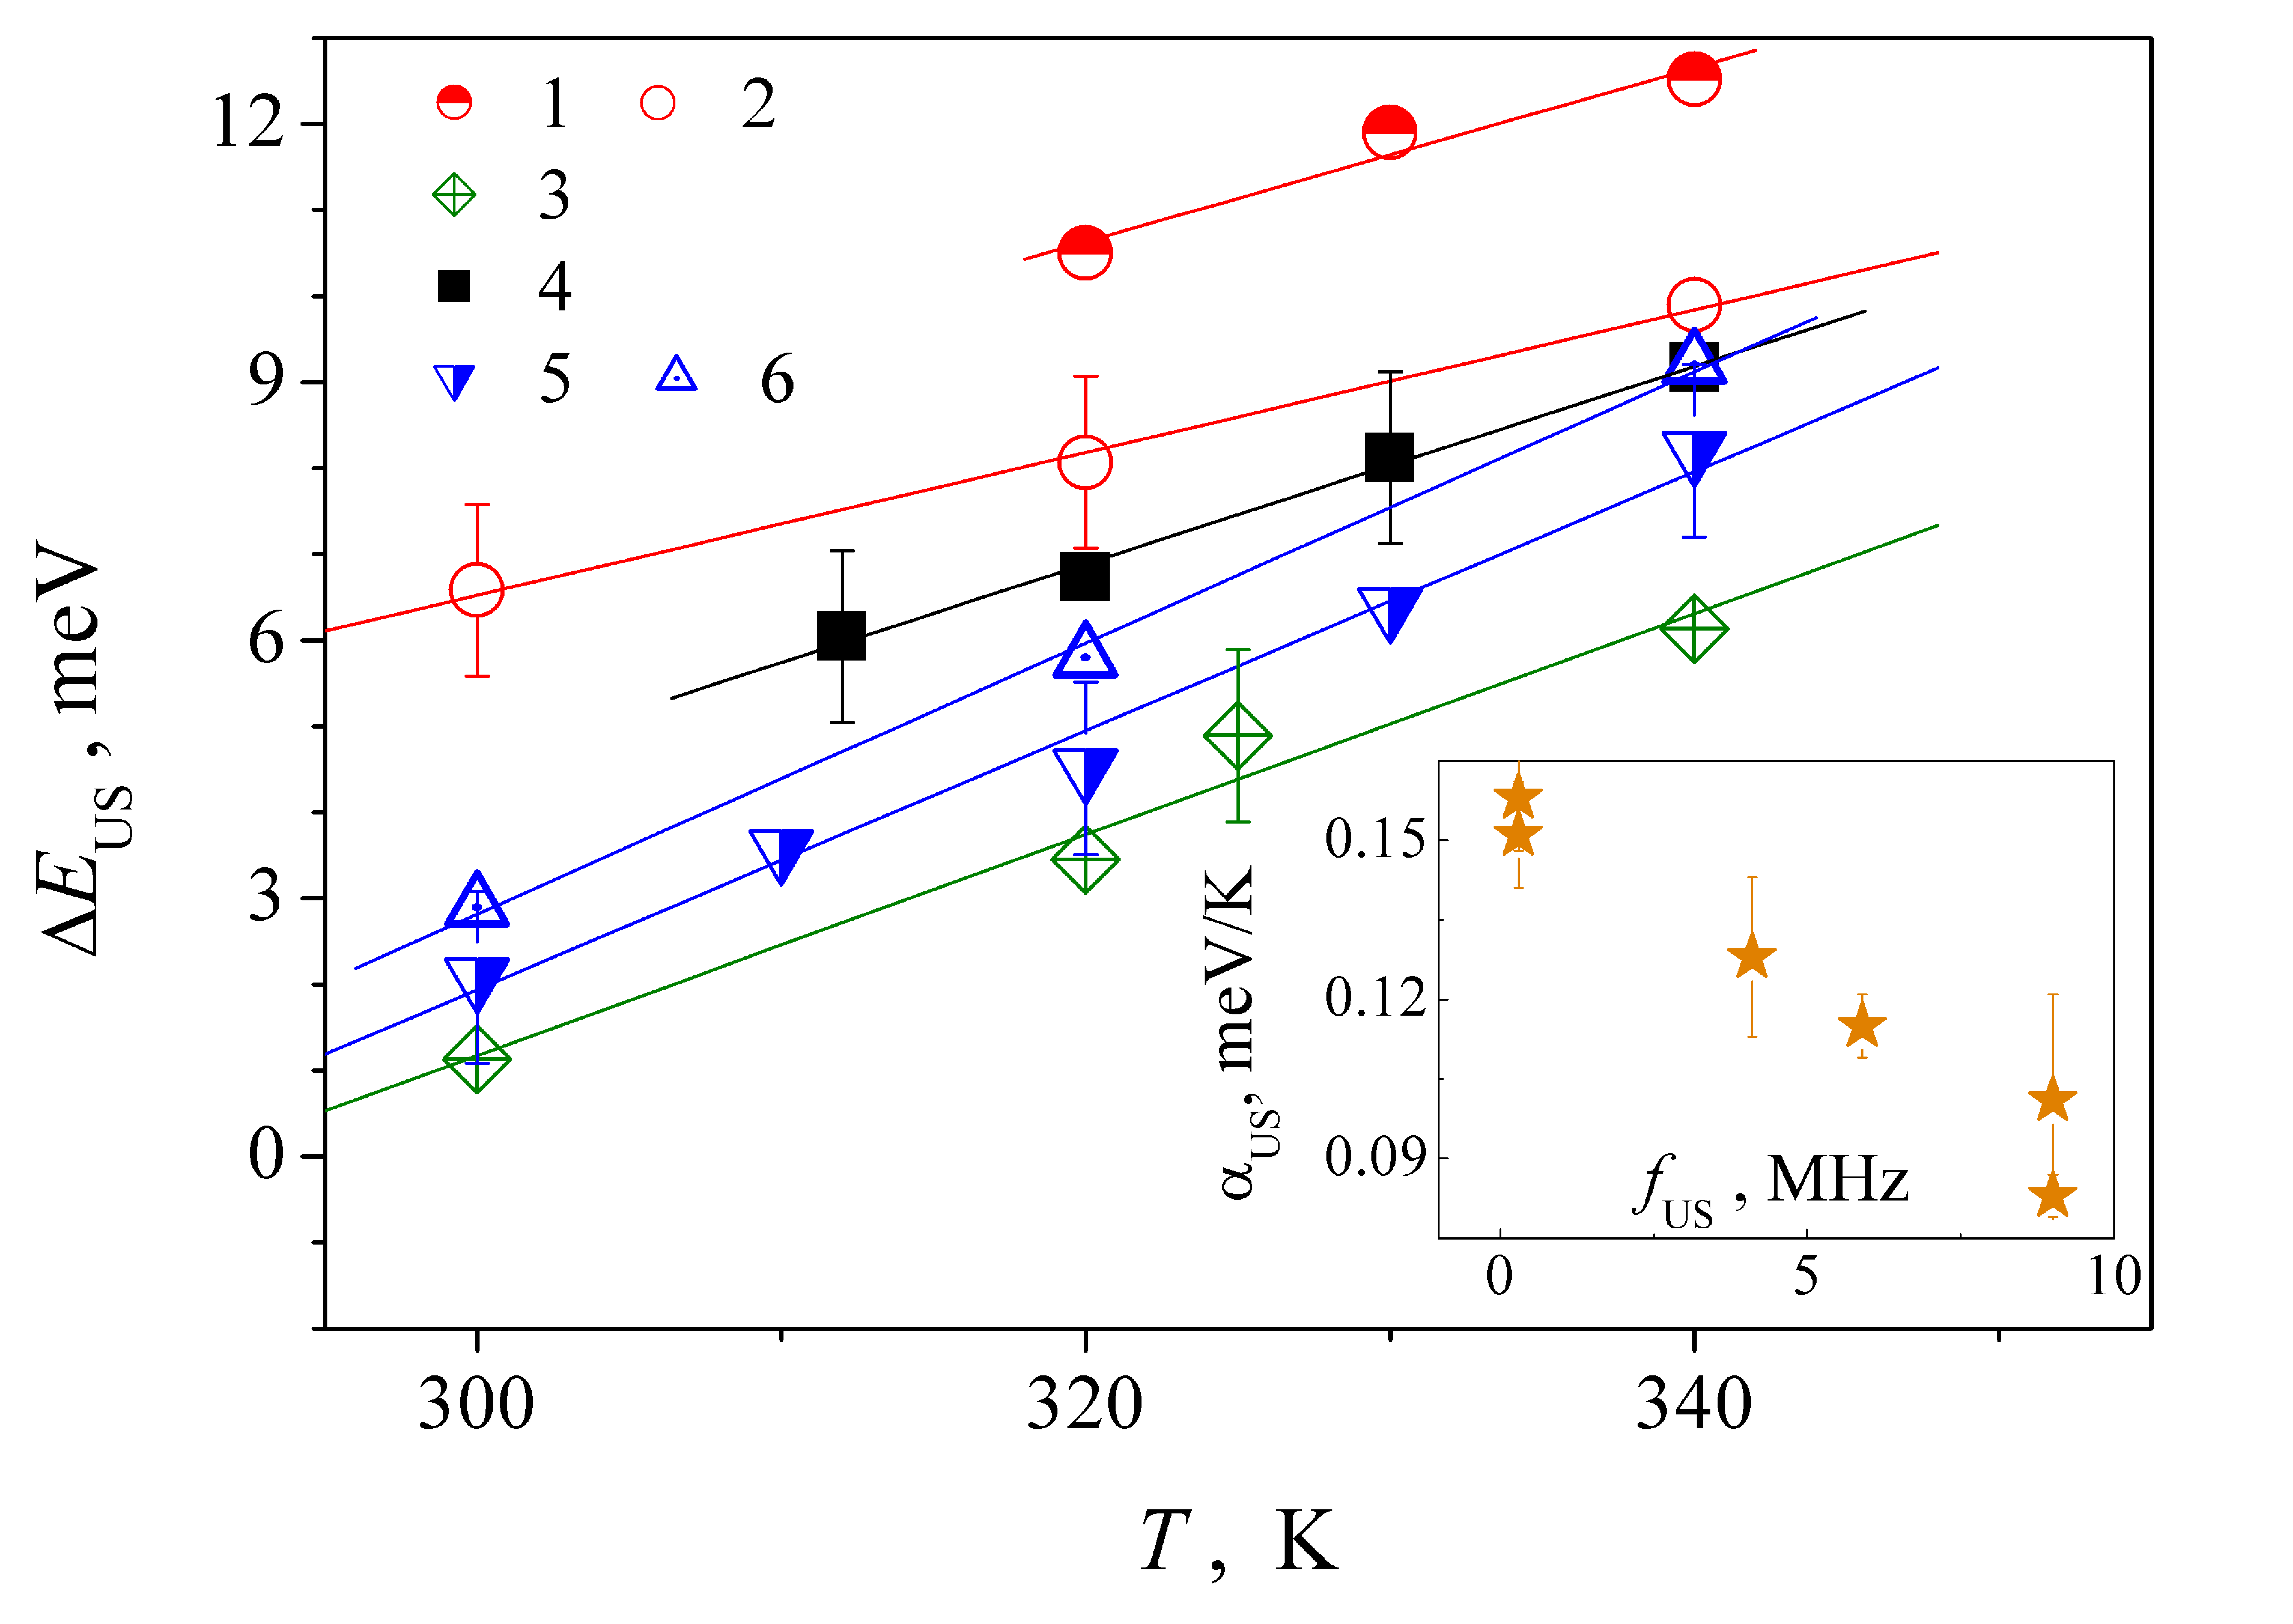
\includegraphics[width=0.45\textwidth]{Fig6}% Here is how to import EPS art
\caption{\label{Fig:EmT}
Temperature dependencies of $\Delta E_\mathrm{US}$.
$N_\mathrm{Fe,tot}$, $10^{13}$~cm$^{-3}$:
3.0 (curve 1 and 2), 4.3 (3), 1.9 (4).
$f_\mathrm{US}$, MHz: 9.0 (1,2), 4.1 (3), 5.9 (4), 0.3 (5,6).
$W_\mathrm{US}$, W/cm$^2$: 1 (1), 0.87 (2), 0.48 (3), 1.0 (4), 0.58 (5), 0.76 (6).
The marks are the experimental results, the lines are the linear fitted curves.
Inset: Frequency dependence of temperature coefficient $\Delta E_\mathrm{US}$.
}
\end{figure}

\subsection{\label{sec:Meh} Possible mechanisms of ultrasound influence}

It is obvious that the analysis of the possible reasons for US impact should be based on the mechanisms of iron-related defect transformation.
It is suggested that FeB pair dissociation is a two-staged process \cite{FeBAssJAP2014,FeBLight2,KIMERLINGFeB}.
First, the electron capture process leads to Fe$_i^+$ neutralization, which removes the Coulombic attraction between Fe$_i^0$ and B$_s^-$.
Second, the electron capture results in the deposition of diffusion barrier energy and spatial dissociation of atoms.
In the literature, two possibilities are discussed:
the second capture, which leads to negative charge state (Fe$_i^-$) and consequently to Coulombic repulsion of Fe$_i^-$B$_s^-$ pair,
and the second capture, which deposits the necessary Fe$_i^0$ migration energy
after recombination with a hole.
The second way is known\cite{FeBAssJAP2014} as recombination-enhanced defect reaction (REDR) and is caused by a strong electron-lattice coupling at the defect.

As for the association, it happens due to Fe$_i^+$ field-assisted migration to B$_s^-$.
Therefore, a more detailed expression for $\tau_\mathrm{ass}$ takes
the following form \cite{FeBAssJAP2014,FeBJAP2005,FeBKin2019}:
\begin{equation}
\label{eqTass2}
\tau_\mathrm{ass}=\frac{\varepsilon\varepsilon_0 kT}{q^2D_\mathrm{Fe}N_A}=
\frac{\varepsilon\varepsilon_0 kT}{q^2D_\mathrm{0,Fe}N_A}\exp\left(\frac{E_m}{kT}\right)\,,
\end{equation}
where
iron diffusivity
$D_\mathrm{Fe}=D_\mathrm{0,Fe}\exp(-E_m/kT)$,
and in the general case\cite{AZIZ2001,Stavola,WeberFe}
$D_\mathrm{0,Fe}=\beta\nu a_0^2\exp(\delta S_\mathrm{Fe}/k)$,
$\beta$ is the correlation factor,
$\nu$  is the effective vibrational (attempt) frequency,
$a_0$ is the jump distance,
$\delta S_\mathrm{Fe}$ is the migration entropy.

For non-piezoelectric materials,
the main effect of acoustic waves is associated with the mechanical stresses they cause.
It is reported \cite{AZIZ2001,AzizPhysRev,FeStrain,MirzadeJAP2011,MirzadeJAP2008,PeleshchakUJF2016,Pavlovich,Krevchik} about several stress-related mechanisms of impurity diffusivity variation.
For instance, Aziz \emph{et al.} \cite{AZIZ2001,AzizPhysRev} show that due to static stresses
$\sigma_\mathrm{stat}$ in the crystal,
the impurity migration energy can decrease by
$\Delta E=\sigma_\mathrm{stat}V^\ast$,
where $V^\ast$ is the activation strain tensor.
It is known\cite{Yost} that as US propagates through the crystal,
it causes static strain:
\begin{equation}
\label{eqUstat}
u_\mathrm{stat}=\frac{\beta}{8}\left(\frac{2\pi f_\mathrm{US}u_\mathrm{US}}{\upsilon_\mathrm{US}}\right)^2
=\frac{\beta W_\mathrm{US}}{4\rho_\mathrm{Si}\upsilon_\mathrm{US}^3}\,,
\end{equation}
where
$\beta$ is the acoustic nonlinearity parameter,
$u_\mathrm{US}=\frac{1}{\pi f_\mathrm{US}}\sqrt{\frac{W_\mathrm{US}}{2\rho_\mathrm{Si}\upsilon_\mathrm{US}}}$
is the amplitude of lattice atom displacements.
Therefore, the effect should be linear with respect to the US intensity, which correlates with the experimental data.
It is known \cite{AzizPhysRev,Chen2006}, however, that $V^\ast=(0.01-0.2)\Omega$,
where
$\Omega$ is the atomic volume ($\sim2\cdot10^{-29}$~m$^3$ for silicon),
and the value of the multiplier depends on the kind of impurity.
If we consider the propagation of longitudinal waves in direction [100]
($\beta=2.0003$ is assumed\cite{NelinSi}, $\sigma_\mathrm{stat}=c_{11} u_\mathrm{stat}$,
$c_{11}=166$~GPa),
for $W_\mathrm{US}=1$~W/cm$^2$  we shall obtain $\Delta E=5\cdot10^{-11}$~eV.
Therefore, this mechanism cannot be the cause of the revealed effect.

According to the data \cite{MirzadeJAP2011,MirzadeJAP2008,PeleshchakUJF2016}, the diffusion of impurities in US fields can occur due to elastic deformation.
In particular, the energy of interaction between a single defect and the strain field is given by
\begin{equation}
\label{eqEint}
E_\mathrm{int}(x,t)=-K\Omega_d\xi(x,t)\,,
\end{equation}
where $K$ is the bulk modulus (102~GPa for Si),
$\Omega_d$ is the variation of crystal volume, in the result of point defect formation,
for interstitial defect \cite{MirzadeJAP2008} $\Omega_d=(1.7-2.2)\Omega$,
$\xi$ is the lattice \textcolor[rgb]{0.00,0.07,1.00}{\uline{relative}} deformation by the acoustic wave.
The estimation of maximum interaction for
$W_\mathrm{US}=1$~W/cm$^2$ yields $E_\mathrm{int}\simeq~0.1$~meV.
And although Baransky \emph{et al.} \cite{BaranskyPSS} state that in case of clusters containing $N_t$ defects, a collective effect can be observed, when $E_\mathrm{int}\rightarrow N_t E_\mathrm{int}$,
in our opinion, this mechanism cannot be crucial in the effect of AI acceleration of  FeB pair association revealed in our research.

In turn, the most probable cause of a decrease in $\tau_\mathrm{ass}$ is the process of impurity interactions with nonequilibrium excitations of the crystal lattice described in
Refs.~\onlinecite{Pavlovich,Krevchik},
which results in the change in probability of diffusion transitions.
According to Pavlovich \cite{Pavlovich},
the US influence \textcolor[rgb]{0.00,0.07,1.00}{\uline{is that it causes}} the increase of crystal effective temperature and effective decrease of ``polaron'' activation energy.
The latter is related to the transfer of lattice deformation around the impurity during diffusion transition \cite{Pavlovich}.
It should be noted that according to calculations \cite{Pavlovich}, this effect should depend linearly on US intensity and temperature,
which correlates with experimentally found peculiarities of AI changes.
In addition, according to Krevchik \emph{et al.} \cite{Krevchik},
$\Delta E_\mathrm{US}\sim t_s$,
where $t_s$ is phonon collision time, which can account for the revealed frequency dependence of the effect.

\textcolor[rgb]{0.00,0.07,1.00}{\uline{
It should be noted that the iron boron pairs are found\cite{Ostapenko1995,Ostapenko1994APL,Ostapenko1995SST}
to dissociate due to ultrasound treatment.
In our opinion,
the reported herein and previous results have a lot in common.
In fact, according to Ostapenko \emph{et al.}\cite{Ostapenko1995SST}
Fe$_i$ has to ``jump'' to the next nearest interstitial under ultrasound action;
we state about the decrease in Fe$_i$ migration energy value
as well as the enhance of Fe$_i$ diffusivity
in case of ultrasound loading.
Further, the efficiency of AI dissociation, as well as AI $\tau_\mathrm{ass}$ fall, increases
with the rise of temperature.
The difference in the action of ultrasound
(the iron-boron pairs dissociation or the enhancing of pairing)
is associated with the difference in the intensity of the acoustic influence.
For instance, the researchers used acoustic strain $\xi_\mathrm{US}=10^{-5}$-$10^{-4}$
was used\cite{Ostapenko1995}
to dissociate FeB pairs in Cz--Si.
Furthermore,
Ostapenko and Bell\cite{Ostapenko1995} regarded the resonance condition of
pair reorientation (first step of dissociation) and used $25$-$70$~kHz.
In our case,  $\xi_\mathrm{US}<2\cdot10^{-6}$ and $f_\mathrm{US}=2$-$30$~MHz are deficient to effectively overcome the Coulombic attraction between Fe$_i^+$ and B$_s^-$.
Additionally, the presented data show that the effectiveness of acoustically--induced change
decreases as the ultrasound frequency increases.
Besides, it should be noted that Ostapenko \emph{et al.}\cite{Ostapenko1994APL} asserted
that in the  case  of predominant  dissociated  pairs,  the ultrasound treatment may promote  the
pairing reaction in contradistinction to the case of high fraction of paired iron.
In our case, the predominant  dissociation was realized by intense illumination, and then
the ultrasound loading accelerated pairing.
Thus, the reported results provided empirical evidence  for the above-mentioned prediction.
}}

As far as dissociation is concerned, it is worth paying attention to the possible  US impact on the processes of charge carrier capture.
For instance,  it is suggested \cite{Olikh2018JAP} that in conditions of USL the capture cross sections for complex defects should change because of the change in effective distance between the components.
In particular, this effect is expected to be especially substantial for the complexes whose components have $\Omega_d$ with opposite signs.
This is what is observed for FeB ($\Omega_d(\mathrm{Fe}_i)>0$, $\Omega_d(\mathrm{B}_s)<0$)
and for this reason, the complex should be acoustically active in terms of charge carrier capture.
However, in our opinion, the processes of AI changes in $\sigma_{n(p)}$ should have influenced,
first of all, the characteristic time of dissociation,
but actually, the effects of this kind have not been revealed.
AI increase of $R_a$ should decrease $N_\mathrm{Fe,fit}$ (see Eqs.~(\ref{eqNfe0Exp}),(\ref{eqNfeill})),
however this effect is leveled by the essential difference between $\tau_\mathrm{dis}$
and $\tau_\mathrm{ass}$.
Therefore, probably because of this reason, the US produces an impact on the second stage of dissociation.
On the one hand, Korotchenkov and Grimmeiss show\cite{Korotchenkov1995} that due to the change of impurity location concerning surrounding atoms in silicon under USL,
the activation thermal energy of the carrier captured by the defect  is decreased
(up to about 10~meV at US intensities commensurate to those in our experiments).
A similar increase of electron emission in our case should decrease the equilibrium part of negatively charged Fe ions experiencing Coulombic repulsion with $B_s^-$.
On the other hand, it is shown\cite{OlikhPSS} that USL of low intensity makes some part of the FeB pairs get rearranged in a metastable configuration with a different (orthorhombic) symmetry,
in which the distance between the components is  greater.
At over threshold US intensities, the spatial separation of this kind results in a complete pair dissociation.\cite{Ostapenko1995,Ostapenko1995SST,Ostapenko1994APL}
For our case, however, the important thing is that the decrease in distance weakens the Coulombic repulsion.
\textcolor[rgb]{0.00,0.07,1.00}{\uline{
In addition, the decrease in the concentration of pairs, which dissociate under illumination in the USL case, can be connected to a partial acoustically-induced FeB dissociation.
In fact, if some pairs were dissociated by  ultrasound waves, which had been pre-exited
in the sample with a high initial  fraction of paired Fe,
they can not be dissociated under illumination.
The decrease in the temperature  or photon quantity leads to reduction in the set of FeB which was modified by ultrasound,
or in the set of FeB which was modified by the capture of light-induced electrons, respectively.
The sets cease to overlap and $N_\mathrm{Fe,fit}(W_\mathrm{US}>0)\simeq N_\mathrm{Fe,fit}(W_\mathrm{US}=0)$ --- see Table~\ref{tabSample}.}}
Finally, USL can be the cause of weakening the electron-lattice coupling at the defect as well as the REDR process as a whole.

Numerous publications, see for example Refs.~\onlinecite{LaineIEEEPV2016,FeB:Vahanissi,Teimuraz2014JAP}, report that during such technological processes as temperature stimulated diffusion of dopants or the formation of an antireflection coating,
iron atoms also undergo gettering.
This is caused by Fe ions diffusion to various stocks.
When performed in the US field, these processes, \textcolor[rgb]{0.00,0.07,1.00}{\uline{as the obtained results suggest}},
should  improve the gettering effectiveness because of the greater volume from which
Fe ions could be piled at the stocks.

\section{Conclusion}
The experimental research of ultrasound impact on the processes of FeB pair transformation was carried out in silicon $n^+$-$p$-$p^+$ structures at near room temperatures.
The investigation has revealed an acoustically driven decrease in the portion of FeB pairs that dissociate under the action of light as well as the decrease in Fe ion migration energies.
The latter effect depends linearly on ultrasound intensity;
the temperature decrease and ultrasound frequency increase reduce the acoustically induced change of migration energy.
The analysis has shown that these phenomenons are caused by the interaction of impurities with nonequilibrium excitations of a crystal lattice,  and acoustically driven attenuation of Coulombic repulsion, which is caused by the increase in distance between pair components and/or change in defect's charge.
Thus, ultrasound can be an effective  tool for controlling silicon structure characteristics.


\begin{acknowledgments}
The authors would like to acknowledge the financial supports by National Research Foundation  of Ukraine
(project number 2020.02/0036)
\end{acknowledgments}

\section*{Data Availability Statement}

The data that support the findings of this study are available from the corresponding author upon reasonable request.

%AIP Publishing believes that all datasets underlying the conclusions of the paper should be available to readers. Authors are encouraged to deposit their datasets in publicly available repositories or present them in the main manuscript. All research articles must include a data availability statement stating where the data can be found. In this section, authors should add the respective statement from the chart below based on the availability of data in their paper.
%
%\begin{center}
%\renewcommand\arraystretch{1.2}
%\begin{tabular}{| >{\raggedright\arraybackslash}p{0.3\linewidth} | >{\raggedright\arraybackslash}p{0.65\linewidth} |}
%\hline
%\textbf{AVAILABILITY OF DATA} & \textbf{STATEMENT OF DATA AVAILABILITY}\\
%\hline
%Data available on request from the authors
%&
%The data that support the findings of this study are available from the corresponding author upon reasonable request.
%\\\hline
%Data available in article or supplementary material
%&
%The data that support the findings of this study are available within the article [and its supplementary material].
%\\\hline
%Data openly available in a public repository that issues datasets with DOIs
%&
%The data that support the findings of this study are openly available in [repository name] at http://doi.org/[doi], reference number [reference number].
%\\\hline
%Data openly available in a public repository that does not issue DOIs
%&
%The data that support the findings of this study are openly available in [repository name], reference number [reference number].
%\\\hline
%Data sharing not applicable – no new data generated
%&
%Data sharing is not applicable to this article as no new data were created or analyzed in this study.
%\\\hline
%Data generated at a central, large scale facility
%&
%Raw data were generated at the [facility name] large scale facility. Derived data supporting the findings of this study are available from the corresponding author upon reasonable request.
%\\\hline
%Embargo on data due to commercial restrictions
%&
%The data that support the findings will be available in [repository name] at [DOI link] following an embargo from the date of publication to allow for commercialization of research findings.
%\\\hline
%Data available on request due to privacy/ethical restrictions
%&
%The data that support the findings of this study are available on request from the corresponding author. The data are not publicly available due [state restrictions such as privacy or ethical restrictions].
%\\\hline
%Data subject to third party restrictions
%&
%The data that support the findings of this study are available from [third party]. Restrictions apply to the availability of these data, which were used under license for this study. Data are available from the authors upon reasonable request and with the permission of [third party].
%\\\hline
%\end{tabular}
%\end{center}

%\appendix

%\section{Appendixes}
%
%To start the appendixes, use the \verb+\appendix+ command.
%This signals that all following section commands refer to appendixes
%instead of regular sections. Therefore, the \verb+\appendix+ command
%should be used only once---to set up the section commands to act as
%appendixes. Thereafter normal section commands are used. The heading
%for a section can be left empty. For example,
%\begin{verbatim}
%\appendix
%\section{}
%\end{verbatim}
%will produce an appendix heading that says ``APPENDIX A'' and
%\begin{verbatim}
%\appendix
%\section{Background}
%\end{verbatim}
%will produce an appendix heading that says ``APPENDIX A: BACKGROUND''
%(note that the colon is set automatically).
%
%If there is only one appendix, then the letter ``A'' should not
%appear. This is suppressed by using the star version of the appendix
%command (\verb+\appendix*+ in the place of \verb+\appendix+).
%
%\section{A little more on appendixes}
%
%Observe that this appendix was started by using
%\begin{verbatim}
%\section{A little more on appendixes}
%\end{verbatim}
%
%Note the equation number in an appendix:
%\begin{equation}
%E=mc^2.
%\end{equation}
%
%\subsection{\label{app:subsec}A subsection in an appendix}
%
%You can use a subsection or subsubsection in an appendix. Note the
%numbering: we are now in Appendix~\ref{app:subsec}.
%
%\subsubsection{\label{app:subsubsec}A subsubsection in an appendix}
%Note the equation numbers in this appendix, produced with the
%subequations environment:
%\begin{subequations}
%\begin{eqnarray}
%E&=&mc, \label{appa}
%\\
%E&=&mc^2, \label{appb}
%\\
%E&\agt& mc^3. \label{appc}
%\end{eqnarray}
%\end{subequations}
%They turn out to be Eqs.~(\ref{appa}), (\ref{appb}), and (\ref{appc}).

%\nocite{*}
\section*{References}
\bibliography{olikh}% Produces the bibliography via BibTeX.

\end{document}
%
% ****** End of file aipsamp.tex ******
